\documentclass[american,man]{apa6}

\usepackage{amssymb,amsmath}
\usepackage{ifxetex,ifluatex}
\usepackage{fixltx2e} % provides \textsubscript
\ifnum 0\ifxetex 1\fi\ifluatex 1\fi=0 % if pdftex
  \usepackage[T1]{fontenc}
  \usepackage[utf8]{inputenc}
\else % if luatex or xelatex
  \ifxetex
    \usepackage{mathspec}
    \usepackage{xltxtra,xunicode}
  \else
    \usepackage{fontspec}
  \fi
  \defaultfontfeatures{Mapping=tex-text,Scale=MatchLowercase}
  \newcommand{\euro}{€}
\fi
% use upquote if available, for straight quotes in verbatim environments
\IfFileExists{upquote.sty}{\usepackage{upquote}}{}
% use microtype if available
\IfFileExists{microtype.sty}{\usepackage{microtype}}{}

% Table formatting
\usepackage{longtable,booktabs}
\usepackage[counterclockwise]{rotating}   % Landscape page setup for large tables
\usepackage{multirow}		% Table styling
\usepackage{tabularx}		% Control Column width
\usepackage[flushleft]{threeparttable}	% Allows for three part tables with a specified notes section
\usepackage{threeparttablex}            % Lets threeparttable work with longtable
\usepackage{longtable}              % Allows tables to break across pages

\ifxetex
  \usepackage[setpagesize=false, % page size defined by xetex
              unicode=false, % unicode breaks when used with xetex
              xetex]{hyperref}
\else
  \usepackage[unicode=true]{hyperref}
\fi
\hypersetup{breaklinks=true,
            pdfauthor={},
            pdftitle={Computational Reproducibility in Archaeological Research: Basic Principles and a Case Study of Their Implementation},
            colorlinks=true,
            citecolor=blue,
            urlcolor=blue,
            linkcolor=black,
            pdfborder={0 0 0}}
\urlstyle{same}  % don't use monospace font for urls

\setlength{\parindent}{0pt}
%\setlength{\parskip}{0pt plus 0pt minus 0pt}

\setlength{\emergencystretch}{3em}  % prevent overfull lines

\setcounter{secnumdepth}{0}
\ifxetex
  \usepackage{polyglossia}
  \setmainlanguage{}
\else
  \usepackage[american]{babel}
\fi

% Manuscript styling
\captionsetup{font=singlespacing,justification=justified}
\usepackage{csquotes}

 % Line numbering
  \usepackage{lineno}
  \linenumbers


\usepackage{tikz} % Variable definition to generate author note

% fix for \tightlist problem in pandoc 1.14
\providecommand{\tightlist}{%
  \setlength{\itemsep}{0pt}\setlength{\parskip}{0pt}}

% Essential manuscript parts
  \title{Computational Reproducibility in Archaeological Research: Basic
Principles and a Case Study of Their Implementation}

  \shorttitle{Basic Computational Reproducibility}


  \author{
          Ben Marwick\textsuperscript{1, 2}  }

  \def\affdep{{""}}%
  \def\affcity{{""}}%

  \affiliation{
    \vspace{0.5cm}
          \textsuperscript{1} Department of Anthropology, University of Washington, Seattle\\
          \textsuperscript{2} Center for Archaeological Science, University of Wollongong, Australia  }


%   \def\affinst{{"init", "Department of Anthropology, University of Washington, Seattle", "Center for Archaeological Science, University of Wollongong, Australia"}}%
%   \def\affstate{{"init", "", ""}}%
%   \def\affcntry{{"init", "", ""}}%

 % If no note is defined give only author information if available
    \note{
    \vspace{1cm}
    Author note

    \raggedright
    \setlength{\parindent}{0.4in}

    \newcounter{author}

%     %       %       \setcounter{author}{0}
%         %           \addtocounter{author}{1, 2}
%         %         \expandafter\edef\csname authorid\endcsname{\theauthor}
%         Ben Marwick, \pgfmathparse{\affdep[\authorid]} \pgfmathresult, \pgfmathparse{\affinst[\authorid]} \pgfmathresult, \pgfmathparse{\affcity[\authorid]} \pgfmathresult, \pgfmathparse{\affstate[\authorid]} \pgfmathresult, \pgfmathparse{\affcntry[\authorid]} \pgfmathresult
%       %     .

                      Correspondence concerning this article should be addressed to Ben Marwick, Department of Anthropology, University of Washington, Seattle. E-mail: \href{mailto:bmarwick@uw.edu}{\nolinkurl{bmarwick@uw.edu}}
                }
  
  \abstract{The use of computers and complex software is pervasive in archaeology,
yet their role in the analytical pipeline is rarely exposed for other
researchers to inspect or reuse. This limits the progress of archaeology
because researchers cannot easily reproduce each other's work to verify
or extend it. Four general principles of reproducible research that have
emerged in other fields are presented. An archaeological case study is
described that shows how each principle can be implemented using freely
available software. The costs and benefits of implementing reproducible
research are assessed. The primary benefit, of sharing data in
particular, is an increased number of citations. The primary cost is the
additional time required to enhance reproduciblity, although the exact
amount is difficult to quantify.}
  
  \usepackage{longtable}
  \usepackage{rotating}
  \usepackage{booktabs}

\begin{document}

\maketitle



\section{Introduction}\label{introduction}

Archaeology, like all scientific fields, advances through rigorous tests
of previously published studies. When numerous investigations are
performed by different researchers and demonstrate similar results, we
hold these results to be a reasonable approximation of a true account of
past human behavior. This ability to reproduce the results of other
researchers is a core tenet of scientific method, and when reproductions
are successful, our field advances. In archaeology we have a long
tradition of empirical tests of reproducibility, for example, by
returning to field sites excavated or surveyed by earlier generations of
archaeologists, and re-examining museum collections with new methods.

However we, like many disciplines, have made little progress in testing
the reproducibility of statistical and computational results, or even
facilitating or enabling these tests (Ince, Hatton, \& Graham-Cumming,
2012; Peng, 2011). The typical contemporary journal article describing
the results of an archaeological study rarely contains enough
information for another archaeologist to reproduce its statistical
results and figures. Raw data are rarely openly and fully provided,
perhaps due to the absence of data-sharing standards that acknowledge
the sensitive nature of much of our data. Similarly, many of the
decisions made in cleaning, tidying, analyzing and visualizing the data
are unrecorded and unreported. This is a problem because as
computational results become increasingly common and complex in
archaeology, and we are increasingly dependent on software to generate
our results, we risk deviating from the scientific method if we are
unable to reproduce the computational results of our peers (Dafoe,
2014). A further problem is that when the methods are underspecified, it
limits the ease with which they can be reused by the original author,
and extended by others (Buckheit \& Donoho, 1995; Donoho, Maleki,
Rahman, Shahram, \& Stodden, 2009; Schwab, Karrenbach, \& Claerbout,
2000). This means that when a new methods paper in archaeology is
published as a stand-alone account (i.e., without any accompanying
software), it is challenging and time-consuming for others to benefit
from this new method. This is a substantial barrier to progress in
archaeology, both in establishing the veracity of previous claims and
promoting the growth of new interpretations. Furthermore, if we are to
contribute to contemporary conversations outside of archaeology (as we
are supposedly well-positioned to do, cf. K. W. Kintigh et al. (2014)),
we need to become more efficient, interoperative and flexible in our
research. We have to be able to invite researchers from other fields
into our research pipelines to collaborate in answering interesting and
broad questions about past societies.

In this paper I address these problems by demonstrating a research
methodology that enables computational reproducibility for archaeology
at the level of a familiar research product, the journal article (Figure
\ref{fig:workflow}). First, I outline the general principles that
motivate this approach. These principles have been derived from software
engineering and developed and refined over the last several years by
researchers in computationally intensive fields such as genomics,
ecology, astronomy, climatology, neuroscience, and oceanography (Stodden
\& Miguez, 2013; G. Wilson et al., 2014). Although the data produced by
some of these disciplines are often used by archaeologists, efforts
towards improving reproducibilty in these fields have seen little uptake
among archaeologists. The principles are ordered by scope, such that the
first principle is applicable to every archaeological publication that
makes claims based on archaeological evidence, the second principle is
applicable to most publications that contain quantitative results, and
the third and fourth principles are most applicable to publications that
report substantial and complex quantitative results. In the second part
of the paper, I describe a case study of a recent archaeological
research publication and its accompanying research compendium. In
preparing this publication I developed new methods for enabling the
reproducibility of the computational results. I describe these methods
and the specific tools used in this project to follow the general
principles. While the specific tools used in this example will likely be
replaced by others a few years from now, the general principles
presented here are tool-agnostic, and can serve as a guide for
archaeologists into the future.

\section{General principles of a reproducible
methodology}\label{general-principles-of-a-reproducible-methodology}

\subsection{Data and code provenance, sharing and
archiving}\label{data-and-code-provenance-sharing-and-archiving}

Perhaps the most trivial principle of reproducible research is making
openly available the data and methods that generated the published
results. This is a computational analogue to the archaeological
principle of artefact provenience. For example, without provenience
information, artifacts are nearly meaningless; without providing data
and code, the final published results are similarly diminished. Making
data and code available enables others to inspect these materials to
evaluate the reliability of the publication, and to include the
materials into other projects, and may lead to higher quality and more
impactful published research (Gleditsch \& Strand, 2003; Heather A.
Piwowar, Day, \& Fridsma, 2007; Wicherts, Bakker, \& Molenaar, 2011).
While might seem a basic principle for reproducible research, current
community norms in archaeology, like many disciplines, do not encourage
or reward the sharing of data and other materials used in the research
leading to journal articles (Borgman, 2012; {B.} {McCullough}, 2007;
Stodden, Guo, \& Ma, 2013; Tenopir et al., 2011). While funding
agencies, such as the US National Science Foundation (NSF), require a
data management plan (DMP) in proposals, and some journals, such as PLOS
ONE and Nature, require data availability statements, none of these
require all archaeologists to make their data available by default
(Begley \& Ioannidis, 2015; Miguel et al., 2014). For archaeology
submissions to the NSF, the DMP recommendations were developed by the
Society of American Archaeologists, rather than from within the NSF
(Rieth, 2013).

It is difficult to prescribe a single approach to making data and other
materials openly available because of the wide variety of archaeological
data, and the diversity of contexts it is collected (K. Kintigh, 2006).
As a general principle that should be applicable in all cases, the
provenance of the data must always be stated, even if the data are not
publicly accessible (for example, due to copyright limitations, cultural
sensitivities, for protection from vandalism, or because of technical
limitations). Where a journal article includes data summaries and
visualizations, the principle is that authors make publicly available
(ie. not \enquote{by request}) the computer files containing the most
raw form possible of the data from which the summaries and plots were
generated (eg. spreadsheets of individual measurement records). This
minimalist approach means that only the data needed to support the
publication should be released, the rest can be kept private while
further work is done without risk of being scooped. The data files
should be archived in an online repository that issues persistent URLs
(such as DOIs), that has a commitment to long-term sustainability (such
as participation in the CLOCKSS scheme, Reich (2008)) and requires open
licenses (such as CC-BY or CC-0) for datasets (Stodden, 2009).
Discipline-agnostic repositories include figshare.com and zenodo.org,
and repositories and data sharing services specifically for
archaeologists include the Archaeological Data Service, the Digital
Archaeological Record, and Open Context (Arbuckle et al., 2014; E. C.
Kansa, Kansa, \& Watrall, 2011).

\subsection{Scripted analyses}\label{scripted-analyses}

The dominant mode of interaction with data analysis tools for many
researchers is a mouse-operated point-and-click interface with
commercial software such as Microsoft's Excel, IBM's SPSS and SAS's JMP
(Keeling \& Pavur, 2007; Thompson \& Burnett, 2012). This method of
interaction is a formidable obstacle to reproducibility because mouse
gestures leave few traces that are enduring and accessible to others (G.
Wilson et al., 2014). Ad hoc edits of the raw data and analysis can
easily occur that leave no trace and interrupt the sequence of
analytical steps (Sandve, Nekrutenko, Taylor, \& Hovig, 2013). While it
is possible for a researcher to write down or even video their
mouse-driven steps for others to reproduce, and this would be an
excellent first step for sharing methods in many cases, these are rather
cumbersome and inefficient methods for communicating many types of
analyses. A second problem with much mouse-driven software is that the
details of the data analysis are not available for inspection and
modification because of the proprietary code of the software (Ince et
al., 2012; Vihinen, 2015). This constrains the transparency of research
conducted with much commercial and mouse-driven software (Hatton \&
Roberts, 1994).

While there are many conceivable methods to solve these problems (such
as writing out all the operations in plain English or making a video
screen-capture of the analysis), currently the most convenient and
efficient solution is to interact with the data analysis tools using a
script (Joppa et al., 2013). A script is a plain text file containing
instructions composed in a programming language that direct a computer
to accomplish a task. In a research context, researchers in fields such
as physics, ecology and biology write scripts to do data ingest,
cleaning, analysis, visualizing, and reporting. By writing scripts, a
very high resolution record of the research workflow is created, and is
preserved in a plain text file that can be reused and inspected by
others (Gentleman \& Temple Lang, 2007). Data analysis using scripts has
additional advantages of providing great flexibility to choose from a
wide range of traditional and cutting-edge statistical algorithms, and
tools for automation of repetitive tasks. Sharing these scripts may also
increase the impact of the published research (Vandewalle, 2012). The
general approach of a scripted workflow to explicitly and unambiguously
carry out instructions embodies the principles of reproducibility and
transparency. Examples of programming languages used for scripting
scientific analyses include R, Python and MATLAB (Bassi, 2007; Eglen,
2009; Jeffrey M. Perkel, 2015; Tippmann, 2014). Among archaeologists who
share code with their publications, R is currently the most widely used
programming language (Bocinsky, 2014; Bocinsky \& Kohler, 2014; Borck,
Mills, Peeples, \& Clark, 2015; Contreras \& Meadows, 2014; E. Crema,
Edinborough, Kerig, \& Shennan, 2014; Drake, 2014; T. S. Dye, 2011;
Guedes, Jin, \& Bocinsky, 2015; K. M. Lowe et al., 2014; Mackay et al.,
2014; Marwick, 2013; Peeples \& Schachner, 2012; S. J. Shennan, Crema,
\& Kerig, 2015).

\subsection{Version control}\label{version-control}

All researchers face the challenge of managing different versions of
their computer files. A typical example, in the simple case of a solo
researcher, is where multiple revisions of papers and datasets are saved
as duplicate copies with slightly different file names (for example,
appending the date to the end of the file name). In a more complex
situation with multiple researchers preparing a report of publication,
managing contributions from different authors and merging their work
into a master document can result in a complex proliferation of files
that can be very challenging to manage efficiently. While this
complexity can be an inconvenience, it can lead to more profound
problems of losing track of the provenance of certain results, and in
the worst cases, losing track of the specific versions of files that
produced the published results (Jones, 2013).

One solution to these problems is to use a formal version control system
(VCS) (Sandve et al., 2013), initially developed for managing
contributions to large software projects, and now used for many other
purposes where multiple people are contributing to one file or
collection of files. Instead of keeping multiple copies of a file, a VCS
separately saves each change to a version control database (known as a
\enquote{commit}, for example, the addition of a paragraph of text or a
chunk of code) along with a comment describing the change. The commit
history preserves a high-resolution record of the development of a file
or set of files. Commits function as checkpoints where individual files
or an entire project can be safely reverted to when necessary. Many VCSs
allow for branching, where alternate ideas can be explored in a
structured and documented way without disrupting the central flow of a
project. Successful explorations can be merged into the main project,
while dead ends can be preserved in an orderly way (Noble, 2009). This
is useful in two contexts, firstly to enable remote collaborators to
work together without overwriting each other's work, and secondly, to
streamline responding questions from reviewers about why one option was
chosen over another because all the analytical pathways explored by the
authors are preserved in different branches in the VCS (Ram, 2013).
Version control is a key principle for reproducible research because of
the transparency it provides. All decision points in the research
workflow are explicitly documented so others can see why the project
proceeded in the way it did. Researchers in other areas of science
currently use Git or Subversion as a VCS (Jones, 2013), often through a
public or private online hosting service such as GitHub, BitBucket or
GitLab.

\subsection{Computational
environments}\label{computational-environments}

Most researchers use one of three operating systems as their primary
computational environment, Microsoft Windows, Apple OS X or Linux. Once
we look beyond the level of this basic detail, our computational
environments diversify quickly, with many different versions of the same
operating system in concurrent use, and many different versions of
common data analysis software in concurrent use. For basic data
analysis, the primary problem here is poor interoperability of file
types from different versions of the same software. But for more complex
projects that are dependent on several pieces of complex software from
diverse sources, it is not uncommon for one of those pieces to change
slightly (for example, when an update is released, a minor configuration
is changed, or because different operating systems causes programs to
behave differently), introducing unexpected output and possibly causing
the entire workflow to fail (Glatard et al., 2015). For example,
computationally intensive analyses often use mathematical functions
based on single-precision floating-point arithmetic whose
implementations vary between software (Keeling \& Pavur, 2007) and
across operating systems. For archaeologists this issue is particularly
relevant to simulation studies. This situation can make it very
challenging to create a research pipeline that will remain reproducible
on any computer other than that of the researcher who constructed it
(and into the future on the same computer, as its component software
changes in ways that are beyond control of the researcher, due to
automatic updates).

At the most general level, the principle that attempts to solve this
problem is to provide a description of how other researchers can
recreate the computational environment of the research pipeline. The
simplest form of this is a list of the key pieces software and their
version numbers, this is often seen in the archaeological literature
where exotic algorithms are used. In other fields, where computationally
intensive methods are more widespread, and software dependencies are
more extensive, more complex approaches have emerged, such as
machine-readable instructions for recreating computational environments,
or providing the entire actual computational environment that the
analysis was conducted in (Dudley \& Butte, 2010; Howe, 2012). Either of
these provides another researcher with an identical copy of the
operating systems and exact versions of all software dependencies. The
ideal solution is to provide both, because providing the actual
environment alone can result in a \enquote{black box} problem where the
specific details of the environment are not available for inspection by
another researcher, and the environment cannot easily be extended or
joined to other environments for new projects. This results in a loss of
transparency and portability, but this can be mitigated by providing a
plain-text file that contains the instructions on how to recreate the
environment in a machine-readable format. With this information
researchers can easily see the critical details of the environment, as
well as efficiently recombine these details into other environments to
create new research workflows. Examples of systems currently used by
researchers to capture the entire environments include virtual machines
(eg. Oracle's VirtualBox) and GNU/Linux containers (eg. Docker). These
environments are designed to be run in an existing operating system, so
a researcher might have a GNU/Linux virtual machine running within their
Windows or OS X computer. Vagrantfiles and Dockerfiles are common
examples of machine-readable plain-text instructions for making virtual
machines to an exact specification. One advantage of using
self-contained computational environment like a virtual machine or
container is that it is portable, and will perform identically whether
it is used on the researcher's laptop or high-performance facilities
such as a commercial cloud computing service (Hoffa et al., 2008). While
these more complex approaches may seem a bridge too far for most
archaeologists, they offer some advantages for collaborating in a common
computing environment (i.e., in a project involving two or more
computers using a virtual machine or container environment can simplify
collaboration), and for working on small-scale iterations of an analysis
prior to scaling up to time-consuming and expensive computations.

To summarize, in this section I have described four general principles
of reproducible research. These principles have been derived from
current efforts to improve computational reproducbility in other fields,
such as as genomics, ecology, astronomy, climatology, neuroscience, and
oceanography. The four principles are: make data and code openly
available and archive it in a suitable location, use a programming
language to write scripts for data analysis and visualiations, use
version control to manage multiple versions of files and contributions
from collaborators, and finally, document and share the computational
environment of the analysis. Researchers following these principles will
benefit from an increase in the transparency and efficiency of their
research pipeline (Markowetz, 2015). Results generated using these
principles will be easier for other researchers to understand, reuse and
extend.

\section{Case study: The 1989 excavation at Madjebebe, Northern
Territory,
Australia}\label{case-study-the-1989-excavation-at-madjebebe-northern-territory-australia}

In this section I describe my efforts to produce a publication of
archaeological research that demonstrates the above principles of
reproducible research. I describe the specific tools that I used,
explain my reasons for choosing these tools, and note any limitations
and obstacles I encountered. Our paper on Madjebebe (Clarkson et al.,
2015) describes familiar types of evidence from a hunter-gatherer
rockshelter excavation - stone artefacts, dates, sediments, mollusks. We
-- the co-authors of the Madjebebe paper and I -- mostly used
conventional and well-established methods of analyzing, summarizing and
visualizing the data. In this example I expect the a typical reader will
recognize the types of raw data we used (measurements and observations
from stone artefacts, dates, sediments, mollusks), and the output of our
analysis (plots, tables, simple statistical test results). The novel
component here is how we worked from the raw data to the published
output. For this Madjebebe publication we experimented with the
principles of reproducible research outlined above, and used data
archiving, a scripted analytical pipeline, version control, and an
isolated computational environment. Additional details of our specific
implementations are available at Marwick (2015).

That standard and familiar nature of the archaeological materials and
methods used in the paper about Madjebebe should make it easy for the
reader to understand how the methods for enhancing reproducibility
described here can be adapted for the majority of research publications
in archaeology. I recognize that not every research project can
incorporate the use of these tools (for example, projects with very
large amounts of data or very long compute times). However, my view is
that the principles and tools described here are suitable for the
majority of published research in archaeology (where datasets are small,
ie. \textless{}10 GB, and analysis compute times are short ie.
\textless{}30 min).

\subsection{Figshare for data
archiving}\label{figshare-for-data-archiving}

We chose Figshare to archive all the files relating to the publication,
including raw data, which we uploaded as a set of CSV files (Figure
\ref{fig:file_structure}). CSV stands for comma separated variables and
is an open file format for spreadsheet files that can be opened and
edited in any text editor or spreadsheet program. Although there are
data repositories designed specifically for archaeologists (Beale, 2012;
Kansa, 2012; eg. Richards, 1997), some of these are fee-based services
and, at the time we deposited our data, they all lacked a programmatic
interface and connections to other online services (such as GitHub, our
version control backup service). Figshare is a commercial online digital
repository service that provides instant free unlimited archiving of any
type of data files (up to 250 MB per file) for individual researchers in
any field, and automatically issues persistent URLs (DOIs). Figshare
also supplies file archiving services for many universities and
publishers, including PLOS and Nature. Figshare allows the user to apply
permissive Creative Commons licenses to archived files that specify how
the files may be reused. We chose the CC0 license for our data files
(equivalent to a release in the public domain), this is widely used and
recommended for datasets (Stodden, 2009). The CC0 license is simpler
than the related CC-BY (requiring attribution) and CC-NC (prohibiting
commercial use) license, so CC0 eliminates all uncertainty for potential
users, encouraging maximal reuse and sharing of the data. We also
archived our programming code on Figshare and applied the MIT license
which is a widely used software license that permits any person to use,
copy, modify, merge, publish, distribute, sublicense and/or sell copies
of the code (Henley \& Kemp, 2008; Morin, Urban, \& Sliz, 2012). Our
motivation for choosing these licenses is to clearly communicate to
others that we are comfortable with our data and code to be reused in
any way - with appropriate attrition (Stodden, 2009). The MIT license
has the added detail of specifically not providing a warranty of any
kind and absolving us as authors from liability for any damages or
problems that others might suffer or encounter when using our code.

\subsection{R for scripting the
analysis}\label{r-for-scripting-the-analysis}

I used the R programming language to script our data analysis and
visualization workflow. I chose R because it is a highly expressive,
functional, interpretive, object-oriented language that was originally
developed by two academic statisticians in the 1990s (J. M. Chambers,
2009; Wickham, 2014). Like Python, R is a free and open source complete
programming language. Where the two differ is that R is heavily
customised for data analysis and visualisation (Gandrud, 2013b; Tippmann
\& others, 2015). Python, which has a reputation for readability and
ease of use, is a general-purpose programming tool with fewer
customisations for data analysis and visualisation (Jeffrey M Perkel,
2015). In the last decade R has acquired a large user community of
researchers, including archaeologists, many of whom contribute packages
to a central open repository that extend the functionality of the
language (Mair et al., 2015). These packages are typically accompanied
by peer-reviewed scholarly publications that explain the algorithms
presented in the package. Such a large and active community means that
many common data analysis and visualization tasks have been greatly
simplified by R packages, which is a key factor in my choice of this
language. For example, rOpenSci is a collective of scientists mostly in
ecology, evolution, and statistics that supports the development of R
packages to access and analyse data, and provide training to researchers
(Boettiger, Hart, Chamberlain, \& Ram, 2015). Our publication depended
on nineteen of these user-contributed packages, which saved me a
substantial amount of programming effort. I also organised our code as a
custom R package because it provides a logical and widely shared
structure to organizing the analysis and data files. The R package
structure gives us access to the many quality control tools involved in
package building, and is a convenient template for projects of any scale
(Wickham, 2015). Because packages are ubiquitous among R users, we hope
that by providing our code as an R package the use of familiar
conventions for organizing the code will make it easier for other users
to inspect, use and extend our code.

The knitr and rmarkdown packages are especially relevant to our efforts
to make our analysis reproducible (Xie, 2013). Knitr provides algorithms
for dynamically converting text and R code into formatted documents
(i.e., PDF, HTML or MS Word) that contain the text and the output of the
code, such as tables and plots. Rmarkdown provides an authoring format
that enables the creation of dynamic documents using a simple syntax
(related to HTML and LaTeX, but simpler) for formatting text and
managing citations, captions and other typical components of a
scientific document (Baumer \& Udwin, 2015; Baumer, Cetinkaya-Rundel,
Bray, Loi, \& Horton, 2014). The rmarkdown package uses a document
formatting language called markdown, which has a simple syntax for
styling text, and extends it into a format called R markdown that
enables embedded computation of R code contained in the markdown
document. Using syntax for styling in markdown (and HTML, LaTeX, etc.)
is different to composing and editing in Microsoft Word because markdown
separates presentation from content. An example of this can be seen in
the heading in figure \ref{fig:literate_programming}, where the two hash
symbols are the syntax for a heading, and the formatting is applied only
when the document is executed. Together, the knitr and rmarkdown
packages enabled us to compose a single plain-text source document that
contained interwoven paragraphs of narrative text and chunks of R code.
This approach has the code located in context with the text so any
reader can easily see the role of the code in the narrative. This
results in an executable paper (cf. Leisch, Eugster, \& Hothorn, 2011;
Nowakowski et al., 2011), which, when rendered by the computer using the
knitr package, interprets the R code to generate the statistical and
visual output and applies the formatting syntax to produce readable
output in the form of a HTML, Microsoft Word or PDF file that contains
text, statistical results and tables, and data visualizations. This
practice of having documentation and code in a single interwoven source
document is known as literate programming (Knuth, 1984). This is a focus
of many efforts to improve the reproducibility of research, for example,
by computer scientists and neuroscientists (Abari, 2012; Delescluse,
Franconville, Joucla, Lieury, \& Pouzat, 2012; Schulte, Davison, Dye, \&
Dominik, 2012; Stanisic, Legrand, \& Danjean, 2015), but is not a
mainstream practice in any field.

\subsection{Git and GitHub for version control and code
sharing}\label{git-and-github-for-version-control-and-code-sharing}

I chose Git as our version control system because it is by far the most
widely used version control system at the moment, both in research
contexts and for software engineering (Jones, 2013; Loeliger \&
{McCullough}, 2012). Git is a free and open source cross-platform
program for tracking changes in plain text documents. The current
popularity of Git is important because it means there is a lot of
documentation and examples available to learn how to use the system. The
key benefit of using Git was saving episodes of code-writing in
meaningful units, for example the preparation of each figure was a
single commit (Figure \ref{fig:git}). This was helpful because if some
new code had an unexpected effect on an earlier figure, I could revert
back to the previous commit where the code worked as expected. This
high-resolution control over the progress of the code-writing provided
by the version control system was helpful for identifying and solving
problems in the analysis. During the peer-review and proofing stages I
used Git commits to indicate the exact version of the code that was used
for the draft, revised and final versions of the paper, which was
helpful for keeping track of the changes we made in response to the
reviewers' comments.

I used GitHub as a remote backup for our project, hosting the code and
data files together with their Git database. GitHub is one of several
commercial online services that hosts Git repositories and provides
online collaboration tools (GitHub repositories that are open to the
public are free, but fees are charged for private repositories;
fee-waivers are available for academic users). While writing the paper,
we worked on a private GitHub repository that was not publicly
accessible because we needed approval from other stakeholders (the
Aboriginal group on whose land the archaeological site is located) of
the final paper before revealing it to the public. When the paper was
published, I made the repository open and publicly available on GitHub
(Barnes, 2010), as well as archiving a copy of the code on Figshare with
the data. The code on Figshare is frozen to match the output found in
the published article, but the code on GitHub continues to be developed,
mostly minor edits and improvements that do not change the contented of
the executed document. GitHub has Git-based tools for organizing
large-scale collaboration on research projects that are widely used in
other fields, but we did not use these because of the small scale of our
project (Gandrud, 2013a).

\subsection{Docker for capturing the computational
environment}\label{docker-for-capturing-the-computational-environment}

Currently there are two widely used methods for creating portable,
isolated computational environments. The most established method is to
create a virtual machine, usually taking the form of a common
distribution of GNU/Linux such as Ubuntu or Debian. Although this is a
widely used and understood method, it is also time-consuming to prepare
the virtual machine, and the virtual machine occupies a relatively large
amount of disk space (8 Gb in our case). We preferred the GNU/Linux
container method because the virtual environment can be created much
faster (which is more convenient for iteration) and the container image
occupies much less disk space. The key difference between the two is
that a virtual machine replicates an entire operating system, while the
container image only shares some of the system resources to create an
isolated computational environment, rather than requiring a complete
system for each environment (Figure \ref{fig:docker}). The low resource
use of the container system makes it possible to run several virtual
environments simultaneously on a Windows or Mac desktop or laptop
computer.

The specific GNU/Linux container system we used is called Docker, and is
currently the dominant open source container system (Boettiger, 2015).
Like Git and R, Docker is a free and open source program. Docker is
developed by a consortium of software companies, and they host an open,
version-controlled online repository of ready-made Docker images, known
as the Docker Hub, including several that contain R, RStudio in the
GNU/Linux operating system. We used images provided by other R users as
our base image, and wrote a Dockerfile to specify further customizations
on this base image. These include the installation of the JAGS library
(Plummer \& others, 2003) to enable efficient Bayesian computation in R.
Our Docker image is freely available on the Docker Hub and may be
accessed by anyone wanting access to the original computational
environment that we used for our analysis. Similarly, our Dockerfile is
included in our code repository so that the exact contents of our Docker
image are described (for example, in case the Docker Hub is unavailable,
a researcher can rebuild our Docker image from the Dockerfile). Using
the Dockerfile, our image can be reconstituted and extended for other
purposes. We treated our Docker image as a disposable and isolated
component, deleting and recreating it regularly to be sure that the
computational environment documented in the Dockerfile could run our
analyses.

\section{Discussion}\label{discussion}

Developing competence in using these tools for enhancing computational
reproducibility is time-consuming, and raises the question of how much
of this is practical for most archaeologists, and what the benefits and
costs might be. Our view is that once the initial costs of learning the
tools is paid off, implementing the principals outlined above makes
research and analysis easier, and has material professional benefits.

Perhaps the best established benefit is that papers with publicly
available datasets receive a higher number of citations than similar
studies without available data. Piwowar et al. (2007) investigated 85
publications on microarray data from clinical trials and found that
papers that archived their data were cited 69\% more often than papers
that did not archive. However, a larger follow-up study by Piwowar and
Vision (2013) of 10,557 articles that created gene expression microarray
data discovered only a 9\% citation advantage for papers with archived
data. Henneken and Accomazzi (2011) analysed 3814 articles in four
astronomy journals and found that articles with links to open datasets
on average acquired 20\% more citations than articles without links to
data. Restricting the sample to papers published in since 2009 in The
Astrophysical Journal, Dorch found that papers with links to data
receiving 50\% more citations per paper per year, than papers without
links to data. In 1,331 articles published in \emph{Paleoceanography}
between 1993 and 2010, Sears (2011) found that publicly available data
in articles was associated with a 35\% increase in citations. While we
are not aware of any studies specifically of archaeological literature,
similar positive effects of data sharing have been described in the
social sciences. In 430 articles in the \emph{Journal of Peace
Research}, articles that offered data in any form, either through
appendices, URLs, or contact addresses were on average cited twice as
frequently as an article with no data but otherwise equivalent author
credentials and article variables (Gleditsch \& Strand, 2003). It is
clear that researchers in a number of different fields following the
first principle of reproducible research benefit from a citation
advantage for their articles that include publicly available datasets.
In addition to increased citations for data sharing, Pienta et al.
(2010) found that data sharing is associated with higher publication
productivity. They examined 7,040 NSF and NIH awards and concluded that
a research grant award produces a median of five publications, but when
data are archived a research grant award leads to a median of ten
publications.

It is also worth noting that the benefits of using a programming
language such as R archaeological analyses extend beyond enhanced
reproducibility. From a practical standpoint, users of R benefit from it
being freely available for Windows, Unix systems (such as Linux), and
the Mac. As a programming language designed for statistics and data
visualization, R has the advantage of providing access to many more
methods than commercial software packages such as Excel and SPSS. This
is due to its status as the lingua franca for academic statisticians
(Morandat, Hill, Osvald, \& Vitek, 2012; Narasimhan \& others, 2005;
Widemann, Bolz, \& Grelck, 2013), which means that R is the development
environment for many recently developed algorithms found in journals
(Bonhomme, Picq, Gaucherel, \& Claude, 2014; eg. D. N. Reshef et al.,
2011), and these algorithms are readily available for archaeologists and
others to use. R is widely known for its ability to complex data
visualisations and maps with few lines of code (Bivand, Pebesma,
Gomez-Rubio, \& Pebesma, 2008; Kahle \& Wickham, 2013; Sarkar, 2008;
Wickham, 2009). Furthermore, our view is that once the learning curve is
overcome, for most analyses using R would not take any longer than
alternative technologies, and will often save time when previously
written code is reused in new projects.

The primary cost of enhancing reproducibility is the time required to
learn to use the software tools. I did not quantify this directly, but
my personal experience is that about three years of self-teaching and
daily use of R was necessary to develop the skills to code the entire
workflow of our case study. Much less time was needed to learn Git and
Docker, because the general concepts of interacting with these types of
programs are similar to working with R (for example, using a command
line interface and writing short functions using flags and arguments). I
expect that most archaeologists could develop competence much quicker
than I did by participating in short training courses such as those
offered by Software Carpentry (G. Wilson, 2014), Data Carpentry (Teal et
al., 2015), rOpenSci (Boettiger et al., 2015), and similar
organisations, or through the use of R in quantitative methods courses.
We did not measure the amount of time required to improve the
reproducibility of our case study article because we planned the paper
to be reproducible before we started the analysis. This makes it
difficult to separate time spent on analytical tasks from time spent on
tasks specifically related to reproducibility. This situation, where the
case study has \enquote{built-in reproducibility} and the additional
time and effort is marginal, may be contrasted with \enquote{bolt-on
reproducibility}, where reproducibility is enhanced only after the main
analysis is complete. In the \enquote{bolt-on} situation, I might
estimate a 50\% increase in the amount of time required for a project
similar to this one. For multi-year projects with multiple teams the
time needed for the bolt-on approach would probably make it infeasable.

The main challenge we encountered using the tools described above in
project was the uneven distribution of familiarity with them across our
team. This meant that much of the final data analysis and visualization
work presented in the publication was concentrated on the team members
familiar with these tools. The cause of this challenge is mostly likely
the focus on point-and-click methods in most undergraduate courses on
data analysis (Sharpe, 2013). The absence of discussion of software in
the key texts on statistics and archaeology ({VanPool} \& Leonard, 2010)
is also a contributing factor. This contrasts with other fields that
where statistical methods and the computational tools to implement them
are often described together (Buffalo, 2015; S. H. D. Haddock \& Dunn,
2011; Scopatz \& Huff, 2015). This makes it difficult for archaeologists
to acquire the computational skills necessary to enable reproducible
research during a typical archaeology degree, leaving only self-teaching
and short workshops as options for the motivated student.

\section{Conclusion}\label{conclusion}

We have outlined one potential standard way for enhancing the
reproducibility of archaeological research, summarized in figure
\ref{fig:workflow}. Our compendium is a collection of files that follows
the formal structure of an R package, and includes the raw data, R
scripts organised into functions and an executable document, a Git
database that includes the history of changes made to all the files in
the compendium, and a Dockerfile that recreates the computational
environment of our analysis. While the exact components of our
compendium will undoubtedly change over time as newer technologies
appear, we expect that the general principles we have outlined will
remain relevant long after our specific technologies have faded from
use.

Two future directions follow from the principles, tools and challenges
that we have discussed above. First, the rarity of archaeologists with
the computational skills necessary for reproducible research (as we
observed on our group) highlights the need for future archaeologists to
be trained as Pi-shaped researchers, rather than T-shaped researchers
(Figure \ref{fig:shapes}). Current approaches to postgraduate training
for archaeologists results in T-shaped researchers with wide-but-shallow
general knowledge, but deep expertise and skill in one particular area.
In contrast, a Pi-shaped researcher has the same wide breadth, but to
have deep knowledge of both their own domain-specific specialization, as
well as a second area of deep knowledge in the computational principles
and tools that enable reproducible research (Faris et al., 2011).

A second future direction is the need to incentivise training in, and
practicing of, reproducible research by changing the editorial standards
of archaeology journals. Although all the technologies and
infrastructure to enhance research reproducibility are already
available, they are not going to be widely used by researchers until
there are strong incentives and a detailed mandate (B. {McCullough} \&
Vinod, 2003; B. {McCullough}, {McGeary}, \& Harrison, 2006, 2008). One
way to incentivise improvements to reproducibility is for journal
editors to require submission of research compendia in place of the
conventional stand-alone manuscript submission (Miguel et al., 2014). A
research compendium is a manuscript accompanied by code and data files
(or persistent links to reputable online repositories) that allows
reviewers and readers to reproduce and extend the results without
needing any further materials from the original authors (Gentleman \&
Temple Lang, 2007; King, 1995). This paper is an example of a research
compendium, with the source files available at
\url{http://dx.doi.org/10.6084/m9.figshare.1563661}, and the case study
paper on Madgebebe is more complex example of a compendium, online at
\url{http://dx.doi.org/10.6084/m9.figshare.1297059}. Requiring
submission of compendia instead of simply manuscripts is currently being
experimented with by journals in other fields (eg. Quarterly Journal of
Political Science, Biostatistics) (B. Nosek et al., 2015; Peng, 2009).
The results of these experiments suggest that changing research
communication methods and tools is a slow process, but they are valuable
to find mistakes in submissions that are otherwise not obvious to
reviewers, and they show that such changes to editorial expectations are
possible without the journal being abandoned by researchers.

Software pervades every domain of research, and despite its importance
in generating results, the choice of tools is very personal (Healy,
2011), and archaeologists are given little guidance in the literature or
during training. With this paper we hope to begin a discussion on
general principles and specific tools to improve the computational
reproducibility of published archaeological research. This discussion is
important because the choice of tools has ethical implications about the
reliability of claims made in publication. Tools that do not facilitate
well-documented, transparent, portable and reproducible data analysis
workflows may, at best, result in irreproducible, unextendable research
that does little to advance the discipline, or, at worst, may conceal
accidents or fraudulent behaviors that impede scientific advancement
(Baggerly \& Coombes, 2009; Herndon, Ash, \& Pollin, 2014; Laine,
Goodman, Griswold, \& Sox, 2007; Lang, 1993; Miller, 2006).

\section{Acknowledgements}\label{acknowledgements}

Thanks to Chris Clarkson, Mike Smith, Richard Fullagar, Lynley A.
Wallis, Patrick Faulkner, Tiina Manne, Elspeth Hayes, Richard G.
Roberts, Zenobia Jacobs, Xavier Carah, Kelsey M. Lowe, and Jacqueline
Matthews for their cooperation with the JHE paper. Thanks to the Mirarr
Senior Traditional Owners, and to our research partners, the Gundjeimhi
Aboriginal Corporation, for granting permission to carry out the
research that was published in the JHE paper, and led to this paper.
Thanks to Kyle Bocinsky and Oliver Nakoinz for their helpful peer
reviews and many constructive suggestions. This research was carried out
as part of ARC Discovery Project DP110102864. I am a contributor to the
Software and Data Carpentry projects and the rOpenSci collective, beyond
this I declare that I have no conflict of interest.

\newpage

\clearpage

\newpage

Tables

\{\fontsize{8pt}{8pt}\selectfont

\begin{longtable}{lp{2cm}p{7cm}p{4cm}}
  \toprule
 & Term & Explanation & More.information \\ 
  \midrule
1 & Concepts &  &  \\ 
   \midrule
2 & open source & Computer code where the source code is available for inspection, and may be freely re-used and distributed. R, Python and GNU/Linux are all open source. & https://opensource.org/osd \\ 
  3 & open access & Access to research products, such as publications and datasets, without financial or copyright barriers, but such that authors have control over the integrity of their work and the right to be acknowledged and cited. One approach is to publish in open access journals, such as PLoS ONE, another approach is to submit manuscripts of published papers to institutional repositories where they are freely available to the public. & http://www.budapestopenaccessinitiative.org/read \\ 
  4 & reproducibility & A study is reproducible if there is a specific set of computational functions/analyses (usually specified in terms of code) that exactly reproduce all of the numbers and data visualisatios in a published paper from raw data. Reproducibiltiy does not require independent data collection and instead uses the methods and data collected by the original investigator. & https://osf.io/s9tya/ \\ 
  5 & replicability & A study is replicated when another researcher independently implements the same methods of data collection and analysis with a new data set.  & http://languagelog.ldc.upenn.edu/nll/?p=21956 \\ 
  6 & provenance & The origin of data and code, including any transformations occurring along the way. &  \\ 
   \midrule
7 & File formats &  &  \\ 
   \midrule
8 & CSV & A common file format for collecting, sharing and archiving tabular data. This is a plain text file where variables (columns) are separated by commas. Thus the name, 'comma separated variables', it is closely related to TSV, 'tab separated variables' & http://www.digitalpreservation.gov/formats/fdd/fdd000323.shtml \\ 
  9 & plain text & A file that contains simple text characters and no formatting (e.g. margins) or embedded images. Use of plain text files is not dependant on specific programs, so they can be created, read, and edited by almost any program, regardless of operating system and computer architecture. Using plain text formats allows a high degree of interoperability between computational environments, and ensures that your files can be read by other people with minimum effort. Most programming script files are plain text files. & http://www.linfo.org/plain\_text.html \\ 
  10 & binary & A file that must be interpreted by a specific program before it is human-readable and editable. For example,  PDF, Microsoft Word doc and Excel xls files are binary files, and can only be read and edited by those programs. Many commercial programs use proprietary binary file formats. This limits their interoperability and archival value. Images, video and audio files are also binary files. &  \\ 
   \midrule
11 & Licenses for data and code &  &  \\ 
   \midrule
12 & CC0 & Public domain, no rights reserved. This license allows for the greatest freedom for reuse. Used for data by major online repositories such as Dryad, Figshare, Zenodo. Good scientific practices assure proper credit is given via citation, which enforced through peer review.  Marking data with CC0 sends a clear signal of zero barriers to reuse. & https://creativecommons.org/licenses/ \\ 
  13 & CC-BY & Allows for reuse only if attribution is given to the author, in the manner specified by the author. Often used for copyrightable materials such as journal articles in open access publications, for example PLOS ONE, BioMed Central, and Nature Communications. &  \\ 
  14 & CC-NC & Allows for reuse only for non-commercial purposes (for example, a Cultural Heritage Management business would not be allowed to use CC-NC data or code). Not recommended for most research output. &  \\ 
  15 & MIT & A license especially for software that places very few restrictions on the use of the software, and disclaims the author of any responsibility for problems arising from others using the software. It is one of the most popular  licenses for open source software. & http://opensource.org/licenses/MIT \\ 
   \midrule
16 & Data archiving &  &  \\ 
   \midrule
17 & DOI & DOI stands for 'digital object identifier', a persistent (but not permanent) label that stores information about the online location of a electronic file. A DOI also includes metadata, for example in the case of journal article it might include the author, title, date of publication, etc. The online location and metadata of a file may change, but its DOI remains fixed. This means that a DOI is generally a more reliable link to an online document than a URL.  & http://www.doi.org/ \\ 
  18 & figshare & A commercial online digital repository where research output can be freely archived and openly accessed. Issues DOIs for individual files or groups of files. & http://figshare.com/ \\ 
  19 & zenodo & Similar to figshare, but a non-profit service operated by European Organization for Nuclear Research (known as CERN) & https://zenodo.org/ \\ 
  20 & tDAR & The Digital Archaeological Record (tDAR) is a  digital repository for the digital records of archaeological investigations. Fees are charged for archiving files, but access to open files is free. & https://www.tdar.org/ \\ 
  21 & Open Context & A data publishing and archiving service. It is aimed at maximising the integration of data with other services (such as maps, media, and other data sets). Similar to tDAR, there are fees to upload but accessing open data is free. & http://opencontext.org/ \\ 
  22 & Archaeological Data Service & An open data repository focused on output from research and commercial archaeology in the UK. There are fees to upload but accessing open data is free. & http://archaeologydataservice.ac.uk/ \\ 
  23 & CLOCKSS & A not-for-profit joint venture between several academic publishers and research libraries to build a sustainable, geographically distributed dark archive with which to ensure the long-term survival of Web-based scholarly publications. & https://www.clockss.org/ \\ 
   \midrule
24 & Document markup languages &  &  \\ 
   \midrule
25 & markdown & A simple, minimal language for formatting plain text files so that they can be converted into richly formatted HTML, PDF and Microsoft Word documents. Scholarly requirements such as citations, captions and cross-referencing can be enabled with a small amount of HTML or LaTeX and use of Pandoc. & http://daringfireball.net/projects/markdown/syntax \\ 
  26 & R markdown & A variant of markdown that extends it to allow chunks of R code to be embedded among the text. This results in a simple system for literate programming. For example, an R markdown document might have several paragraphs of text, then a chunk of R code that generates a figure, then several more paragraphs of text. Suitable for journal-article-length documents that include narrative text and output from statistical analysis.  & http://rmarkdown.rstudio.com/ \\ 
  27 & LaTeX & A complex document preparation system optimised for producing technical and scientific documentation. Suitable for large multi-part documents such as complex journal articles, books and theses. Literate programming with R code interwoven among text is enabled via the knitr package.  & https://latex-project.org \\ 
  28 & pandoc & An open source program for converting documents between a very wide variety of formats. Often used to convert markdown, R markdown and LaTeX documents to HTML (for web publication), PDF and Microsoft Word documents. It is built into RStudio. & http://pandoc.org/ \\ 
   \midrule
29 & Scientific programming &  &  \\ 
   \midrule
30 & script & A plain text file containing instructions for a computer written in a programming language, for example in R or Python &  \\ 
  31 & R & A free and open source programming language with strengths in data analysis and visualisation. Most effective when used in combination with RStudio, a free and open source integrated development environment for R. & https://www.r-project.org/ \\ 
  32 & Python & A free and open source programming language with a reputation for ease of use and being suitable for a wide range of scientific and commercial applications.  & https://www.python.org/ \\ 
  33 & MATLAB & A commercial programming language known for numerical and symbolic computing capabilities. The algorithms are proprietary, which means you cannot easily see the code of the algorithms and have to trust that MATLAB implemented it correctly. The proprietary nature also makes it hard, if not impossible, for others to extend or create tools for MATLAB. & http://www.mathworks.com/products/matlab \\ 
   \midrule
34 & Version control &  &  \\ 
   \midrule
35 & Git & Open source software for version control and collaboration. It can handle any file type, but is most effective on plain text files such as scripts and markdown/LaTeX documents. & https://git-scm.com/ \\ 
  36 & GitHub & A popular commercial web service that provides collaboration tools and free public hosting of files in git repositories. Private repositories are available for a fee. Similar services include GitLab and Bitbucket, both of which have the advantage of unlimited free private repositories.  & https://github.com/ \\ 
  37 & commit & A Git command to record changes in files to the Git repository. A sequence of commits creates a history of how the files have changed during your work on them.  & http://git-scm.com/book/en/v2/Git-Basics-Recording-Changes-to-the-Repository \\ 
   \midrule
38 & Computational environments &  &  \\ 
   \midrule
39 & virtual machine & The use of software to emulate an entire operating system (such as GNU/Linux, Microsoft Windows or Apple OS X) within another computer. For example, you might use a virtual machine to use a GNU/Linux operating system on a laptop where the main operating system is Microsoft Windows. Virtual machines are convienent for reproducing an entire computational environment, but they can consume a lot of hard disk space which makes sharing and archiving challenging.  &  \\ 
  40 & GNU/Linux & A free and open source computer operating system (i.e., an alternative to Microsoft Windows and Apple OS X). Commonly used for scientific computing, internet servers, supercomputers and Android phones and tablets. Popular distributions of GNU/Linux in academia include Ubuntu and Debian. & http://www.linux.org/ \\ 
  41 & Linux container & A system for running multiple isolated Linux systems (containers) on a single Linux control host. Isolation means that the dependencies can be well understood and documented. In a research context, containers are useful for encapsulating the all of the diverse components of a complex data analysis system. Containers take up less disk space than a virtual machine, and so are more efficient for sharing and archiving. & https://linuxcontainers.org/ \\ 
  42 & Docker & A free and open source system that simplifies the creation, use, sharing and archiving of Linux containers. In a research context Docker makes it easy to document and share computational environments so you can ensure that others have exactly the same software versions as you used. & https://www.docker.com/ \\ 
   \midrule
43 & Communities &  &  \\ 
   \midrule
44 & Software Carpentry & An international non-profit volunteer organisation focusing on teaching researchers basic software skills. Prioritises the use of free and open source software tools, encourages researchers to use permissive licenses for their research products. Target audience is novices with little or no prior computational experience.  & http://software-carpentry.org/ \\ 
  45 & Data Carpentry & Similar to Software Carpentry, but focuses more on domain-specific training covering the full lifecycle of data-driven research. & http://www.datacarpentry.org/ \\ 
  46 & rOpenSci & A collaboration of volunteers from academia and industry developing R-based tools for making scientific research, data and publication freely accessible to the public. They also conduct workshops to train researchers to use R and related tools.  & https://ropensci.org/ \\ 
  \caption{Glossary of key terms used in the text} 
\end{longtable}

\}

\clearpage

\newpage

\{\fontsize{8pt}{8pt}\selectfont

\begin{tabular}{lp{4cm}p{10cm}}
  \toprule
 & Degree of reproducibility & Description \\ 
  \midrule
1 & Low reproducibility & The journal article is the only record of the research, with the reader invited to contact the author for more details. \\ 
  2 & Moderate reproducbility & The journal article is accompanied by files of raw data tables in PDF files and supplementary text describing the methods in more detail. \\ 
  3 & High reproducibility & The journal article includes DOIs to an open access repository that contains plain text files (e.g., CSV format) of raw data, version-controlled script files of R or Python code to reproduce the numbers and figures in the article, and a dockerfile that documents the computational environment of the published analysis.  \\ 
   \bottomrule
\end{tabular}

\}

\begin{figure}[h!]
  \caption{Workflow diagram showing key steps and software components. The boxes with a bold outline indicate key steps and tools that enable computational reproducibility in our project}
  \centering
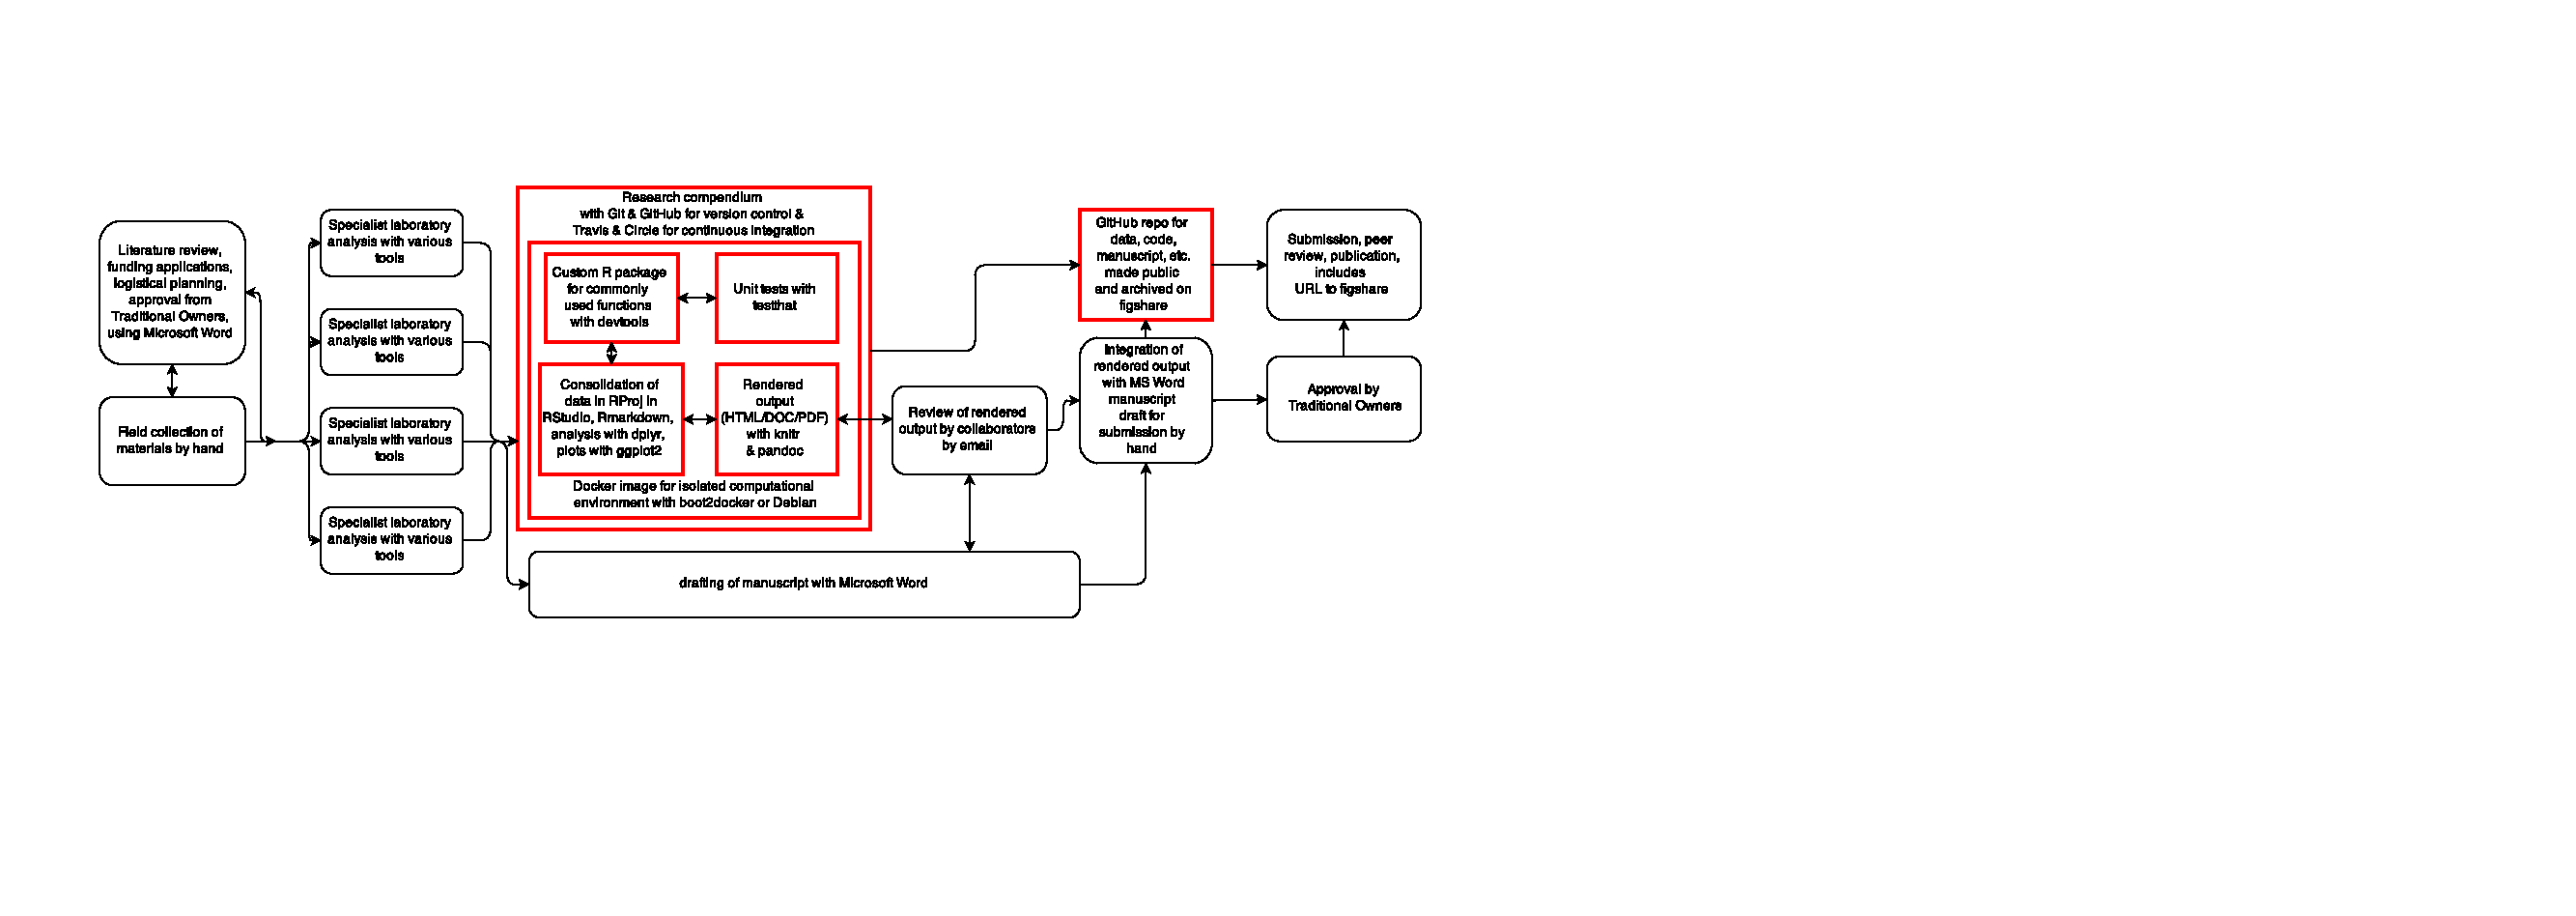
\includegraphics[width=\textwidth]{../figures/figure_workflow.pdf}
\label{fig:workflow}
\end{figure}

\newpage

\begin{figure}[h!]
  \caption{File organisation of the Figshare archive. The items with a dashed border are typical components of an R package, the solid outline indicates custom items added to form this specific compendium, and the shaded items indicate folders and the unshaded items indicate files}
  \centering
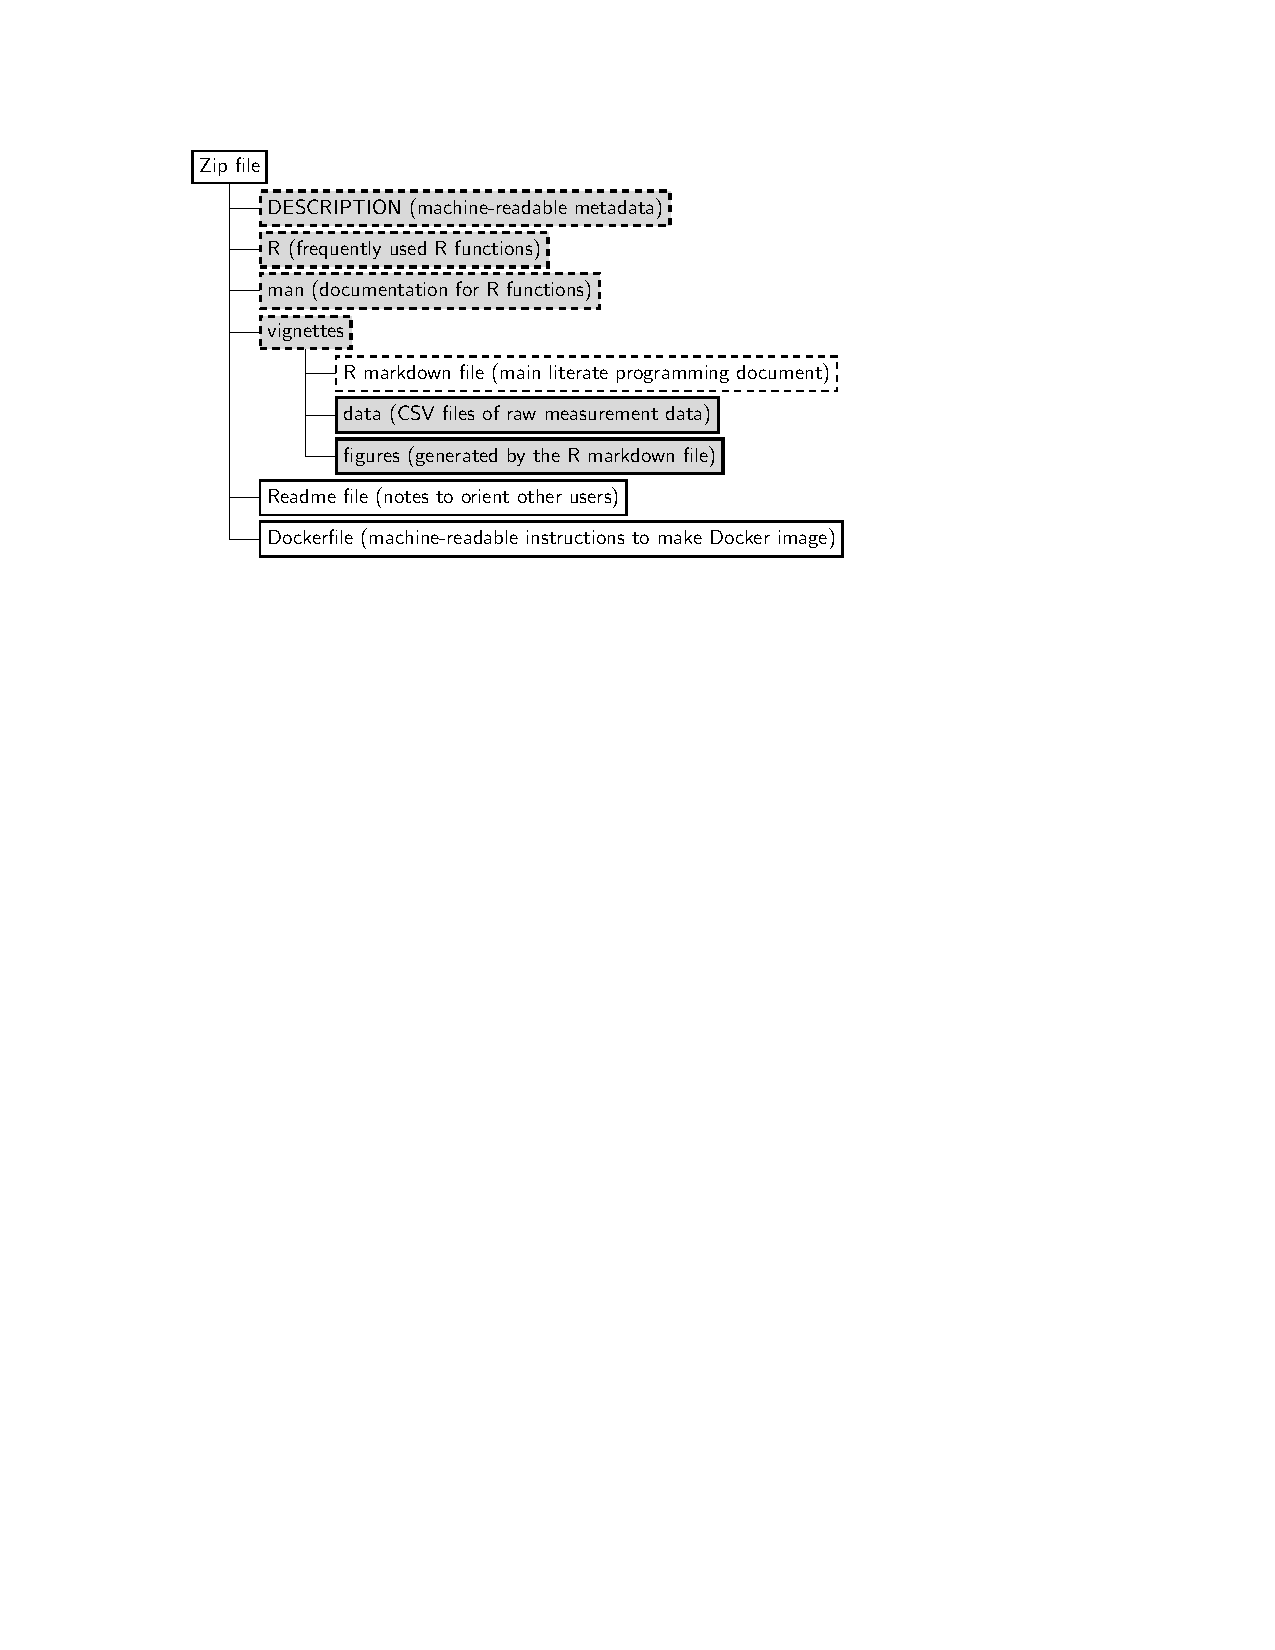
\includegraphics[width=\textwidth]{../figures/figure_compendium_filesystem.pdf}
\label{fig:file_structure}
\end{figure}

\newpage

\begin{figure}[h!]
  \caption{A small literate programming example showing a sample of R markdown script similar to that used in our publication (on the left), and the rendered output (on the right)}
  \centering
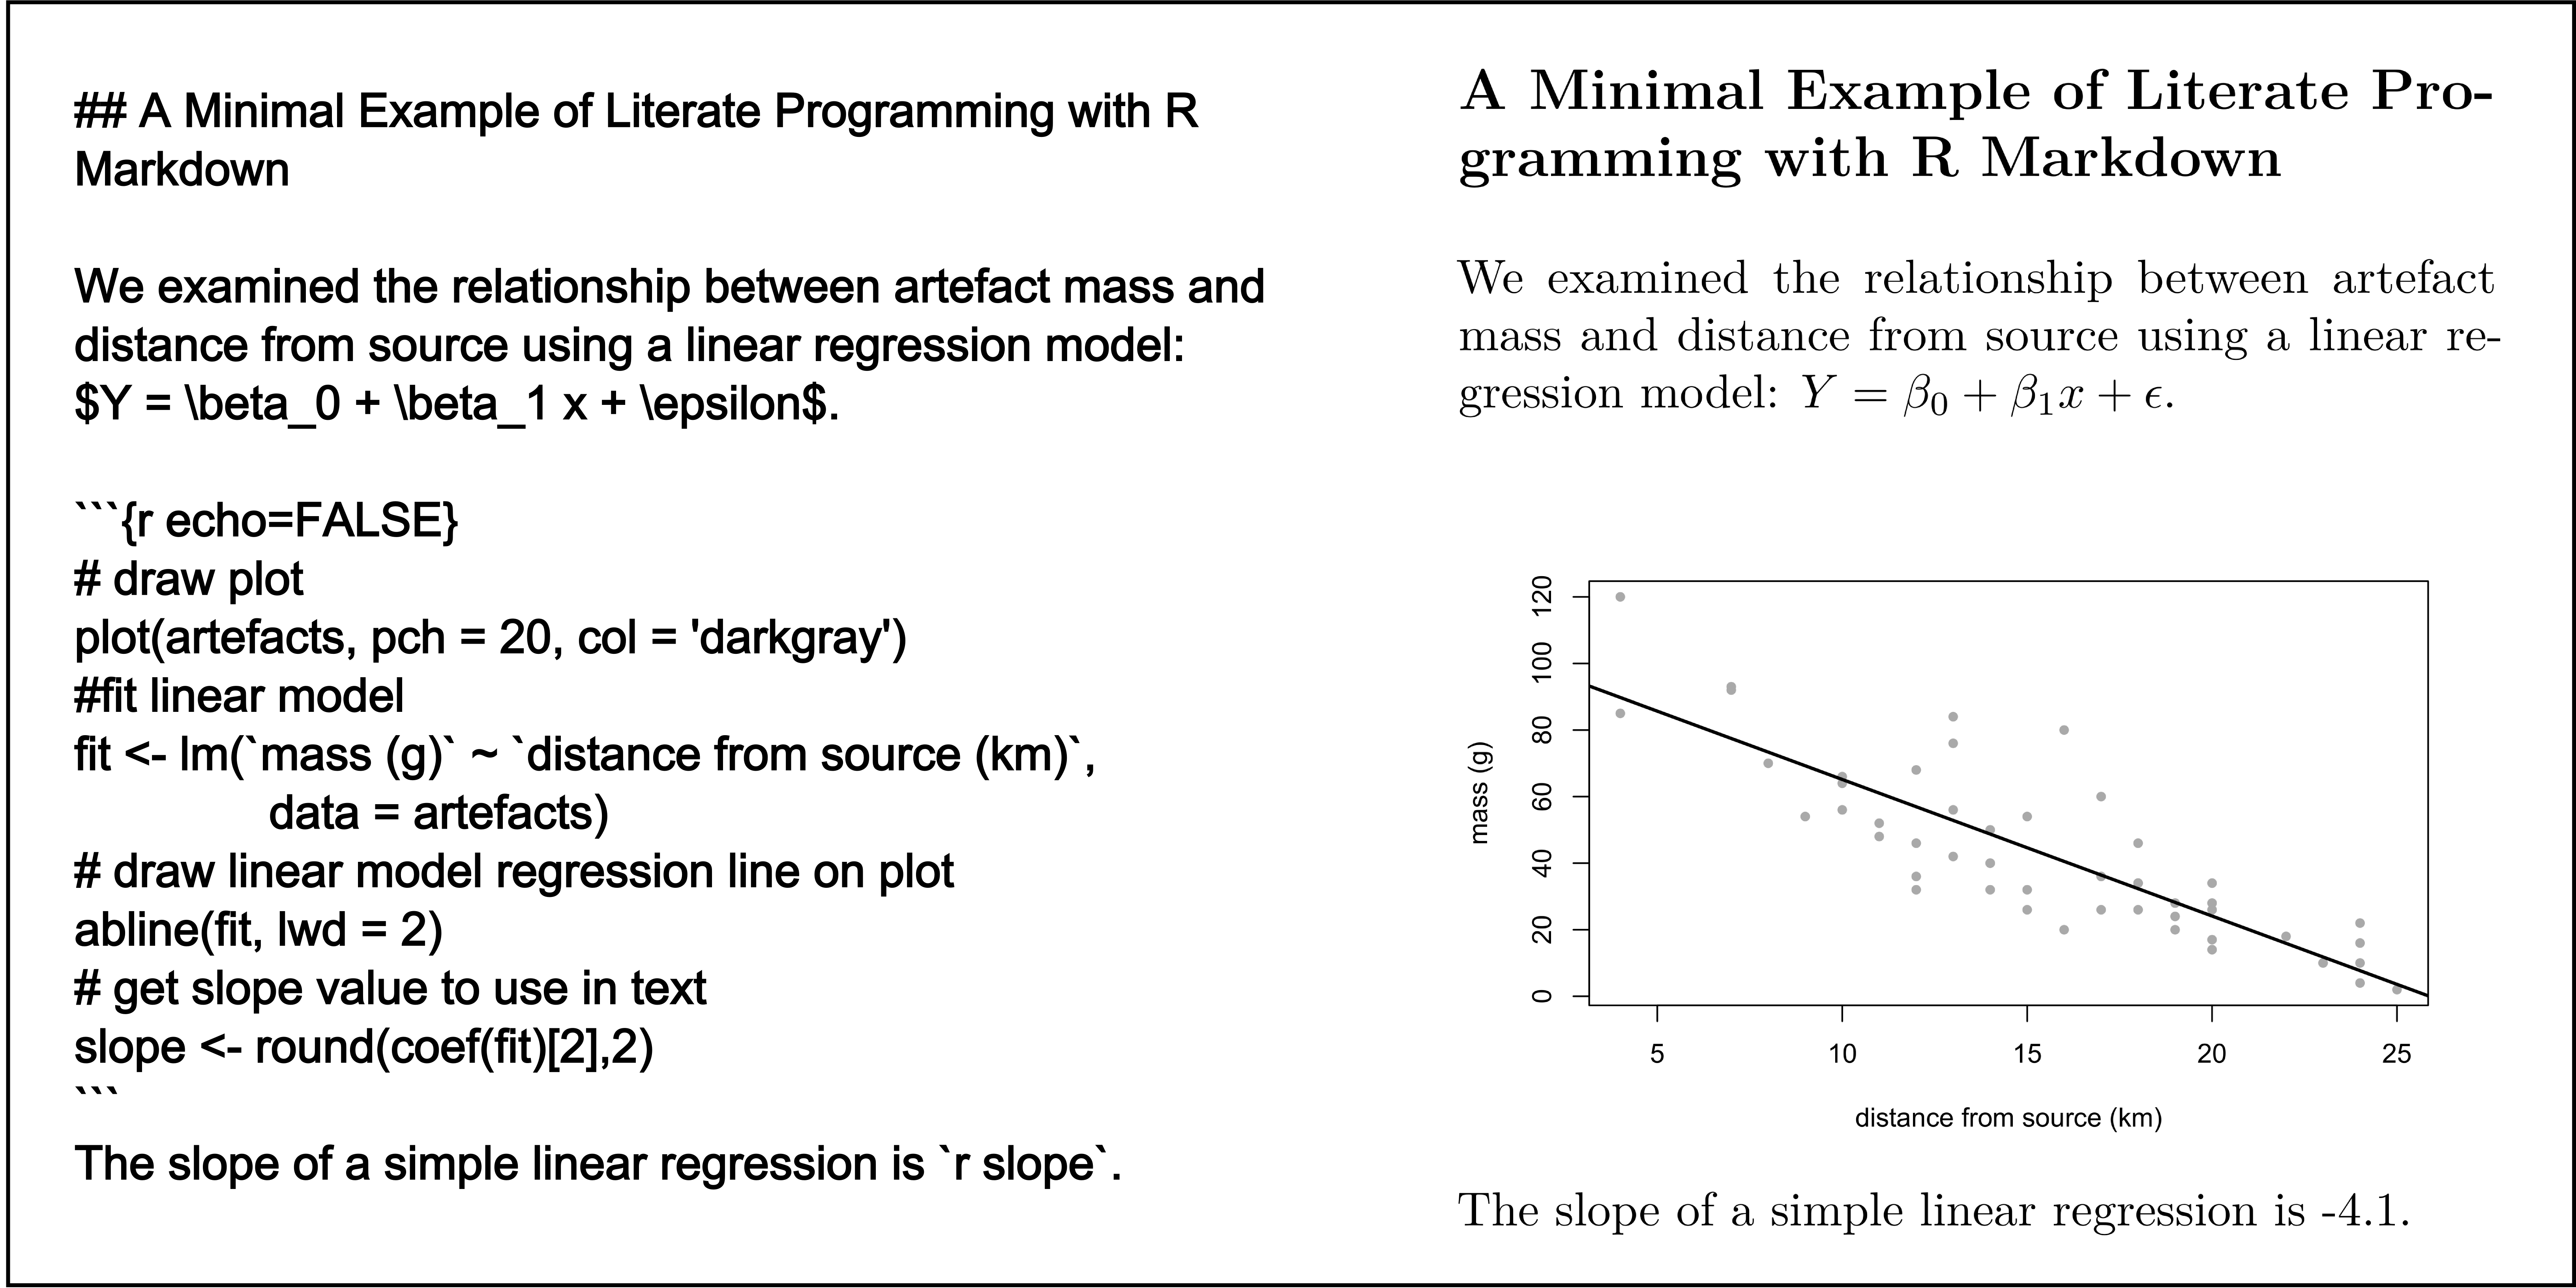
\includegraphics[width=\textwidth]{../figures/figure_literate_programming_example_scource.png}
\label{fig:literate_programming}
\end{figure}

\newpage

\begin{figure}[h!]
  \caption{Git commit history graph. This excerpt shows a typical sequence of commits and commit messages for a research project. The seven character code are keys that uniquely identify each commit. The example here shows the creation and merging of a branch to experiment with a variation of a plot axis.}
  \centering
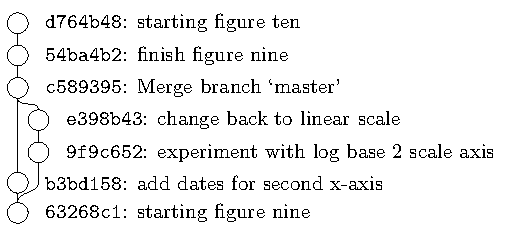
\includegraphics[width=\textwidth]{../figures/figure_git_graph.pdf}
\label{fig:git}
\end{figure}

\newpage

\begin{figure}[h!]
  \caption{Schematic of computer memory use of Docker compared to a typical virtual machine. This figure shows how much more efficiently Docker uses hardware resources compared to a virtual machine. }
  \centering
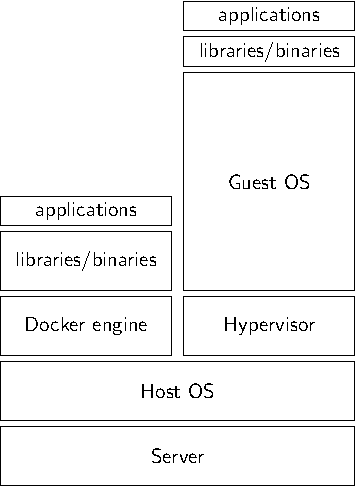
\includegraphics[width=10cm]{../figures/figure_virtual_environments.pdf}
\label{fig:docker}
\end{figure}

\newpage

\begin{figure}[h!]
  \caption{T-shaped and Pi-shaped researchers.}
  \centering
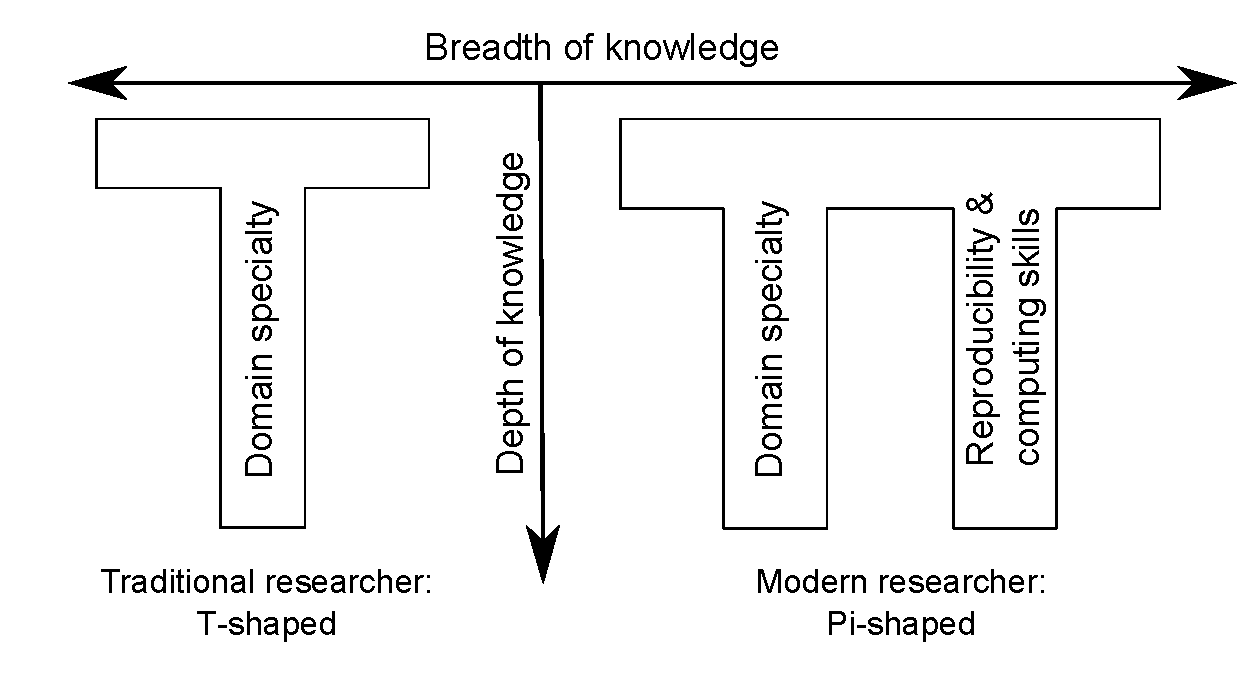
\includegraphics[width=\textwidth]{../figures/figure_t_and_pi_shaped.pdf}
\label{fig:shapes}
\end{figure}

\newpage

\section{References}\label{references}

\setlength{\parindent}{-0.5in} \setlength{\leftskip}{0.5in}
\setlength{\parskip}{8pt}

Abari, K. (2012). Reproducible research in speech sciences.
\emph{International Journal of Computer Science Issues}, \emph{9}(6),
43--52. Retrieved from
\url{http://www.ijcsi.org/papers/IJCSI-9-6-2-43-52.pdf}

Arbuckle, B. S., Kansa, S. W., Kansa, E., Orton, D., Çakırlar, C.,
Gourichon, L., \ldots{} Würtenberger, D. (2014). Data sharing reveals
complexity in the westward spread of domestic animals across neolithic
turkey. \emph{PLoS ONE}, \emph{9}(6), e99845.
doi:\href{http://dx.doi.org/10.1371/journal.pone.0099845}{10.1371/journal.pone.0099845}

Baggerly, K. A., \& Coombes, K. R. (2009). Deriving chemosensitivity
from cell lines: Forensic bioinformatics and reproducible research in
high-throughput biology. \emph{The Annals of Applied Statistics},
1309--1334.

Barnes, N. (2010). Publish your computer code: It is good enough.
\emph{Nature News}, \emph{467}(7317), 753--753.
doi:\href{http://dx.doi.org/10.1038/467753a}{10.1038/467753a}

Bassi, S. (2007). A primer on python for life science researchers.
\emph{PLoS Computational Biology}, \emph{3}(11).
doi:\href{http://dx.doi.org/10.1371/journal.pcbi.0030199}{10.1371/journal.pcbi.0030199}

Baumer, B., \& Udwin, D. (2015). R markdown. \emph{Wiley
Interdisciplinary Reviews: Computational Statistics}, \emph{7}(3),
167--177.
doi:\href{http://dx.doi.org/10.1002/wics.1348}{10.1002/wics.1348}

Baumer, B., Cetinkaya-Rundel, M., Bray, A., Loi, L., \& Horton, N. J.
(2014). R markdown: Integrating a reproducible analysis tool into
introductory statistics. \emph{Technology Innovations in Statistics
Education}, \emph{8}(1). Retrieved from
\url{http://www.escholarship.org/uc/item/90b2f5xh}

Beale, N. (2012). How community archaeology can make use of open data to
achieve further its objectives. \emph{World Archaeology}, \emph{44}(4),
612--633.

Begley, C. G., \& Ioannidis, J. P. A. (2015). Reproducibility in science
improving the standard for basic and preclinical research.
\emph{Circulation Research}, \emph{116}(1), 116--126.
doi:\href{http://dx.doi.org/10.1161/CIRCRESAHA.114.303819}{10.1161/CIRCRESAHA.114.303819}

Bivand, R. S., Pebesma, E. J., Gomez-Rubio, V., \& Pebesma, E. J.
(2008). \emph{Applied spatial data analysis with r} (Vol. 747248717).
Springer.

Bocinsky, R. K. (2014). Extrinsic site defensibility and landscape-based
archaeological inference: An example from the northwest coast.
\emph{Journal of Anthropological Archaeology}, \emph{35}, 164--176.

Bocinsky, R. K., \& Kohler, T. A. (2014). A 2,000-year reconstruction of
the rain-fed maize agricultural niche in the uS southwest. \emph{Nature
Communications}, \emph{5}.

Boettiger, C. (2015). An introduction to docker for reproducible
research. \emph{SIGOPS Oper. Syst. Rev.}, \emph{49}(1), 71--79.
doi:\href{http://dx.doi.org/10.1145/2723872.2723882}{10.1145/2723872.2723882}

Boettiger, C., Hart, T., Chamberlain, S., \& Ram, K. (2015). Building
software, building community: Lessons from the rOpenSci project.
\emph{Journal of Open Research Software}, \emph{1}(1), p.e8.

Bonhomme, V., Picq, S., Gaucherel, C., \& Claude, J. (2014). Momocs:
Outline analysis using r. \emph{Journal of Statistical Software},
\emph{56}(13), 1--24.
doi:\href{http://dx.doi.org/10.18637/jss.v056.i13}{10.18637/jss.v056.i13}

Borck, L., Mills, B. J., Peeples, M. A., \& Clark, J. J. (2015). Are
social networks survival networks? An example from the late pre-hispanic
uS southwest. \emph{Journal of Archaeological Method and Theory},
\emph{22}(1), 33--57.

Borgman, C. L. (2012). The conundrum of sharing research data.
\emph{Journal of the American Society for Information Science and
Technology}, \emph{63}(6), 1059--1078.

Buckheit, J. B., \& Donoho, D. L. (1995). WaveLab and reproducible
research. In A. Antoniadis \& G. Oppenheim (Eds.), \emph{Wavelets and
statistics} (pp. 55--81). Springer New York. Retrieved from
\url{http://link.springer.com/chapter/10.1007/978-1-4612-2544-7_5}

Buffalo, V. (2015). \emph{Bioinformatics data skills reproducible and
robust research with open source tools}. O'Reilly Media, CA. Retrieved
from
\url{http://proxy2.hec.ca/login?url=http://proquestcombo.safaribooksonline.com/?uiCode=hecmontreal\&xmlId=9781449367480}

Chambers, J. M. (2009). \emph{Software for data analysis: Programming
with R} (1st ed. 2008. Corr. 2nd printing 2009 edition.). New York:
Springer.

Clarkson, C., Smith, M., Marwick, B., Fullagar, R., Wallis, L. A.,
Faulkner, P., \ldots{} Florin, S. A. (2015). The archaeology, chronology
and stratigraphy of madjedbebe (malakunanja iI): A site in northern
australia with early occupation. \emph{Journal of Human Evolution},
\emph{83}, 46--64.
doi:\href{http://dx.doi.org/http://dx.doi.org/10.1016/j.jhevol.2015.03.014}{http://dx.doi.org/10.1016/j.jhevol.2015.03.014}

Contreras, D. A., \& Meadows, J. (2014). Summed radiocarbon calibrations
as a population proxy: A critical evaluation using a realistic
simulation approach. \emph{Journal of Archaeological Science},
\emph{52}, 591--608.

Crema, E., Edinborough, K., Kerig, T., \& Shennan, S. (2014). An
approximate bayesian computation approach for inferring patterns of
cultural evolutionary change. \emph{Journal of Archaeological Science},
\emph{50}, 160--170.

Dafoe, A. (2014). Science deserves better: The imperative to share
complete replication files. \emph{PS: Political Science \& Politics},
\emph{47}(01), 60--66.
doi:\href{http://dx.doi.org/10.1017/S104909651300173X}{10.1017/S104909651300173X}

Delescluse, M., Franconville, R., Joucla, S., Lieury, T., \& Pouzat, C.
(2012). Making neurophysiological data analysis reproducible: Why and
how? \emph{Journal of Physiology-Paris}, \emph{106}(3--4), 159--170.
doi:\href{http://dx.doi.org/10.1016/j.jphysparis.2011.09.011}{10.1016/j.jphysparis.2011.09.011}

Donoho, D. L., Maleki, A., Rahman, I. U., Shahram, M., \& Stodden, V.
(2009). Reproducible research in computational harmonic analysis.
\emph{Computing in Science \& Engineering}, \emph{11}(1), 8--18.
doi:\href{http://dx.doi.org/10.1109/MCSE.2009.15}{10.1109/MCSE.2009.15}

Drake, W. H. A. H., Brandon Lee AND Wills. (2014). Strontium isotopes
and the reconstruction of the chaco regional system: Evaluating
uncertainty with bayesian mixing models. \emph{PLoS ONE}, \emph{9}(5),
e95580.
doi:\href{http://dx.doi.org/10.1371/journal.pone.0095580}{10.1371/journal.pone.0095580}

Dudley, J. T., \& Butte, A. J. (2010). Reproducible in silico research
in the era of cloud computing. \emph{Nature Biotechnology},
\emph{28}(11), 1181--1185.
doi:\href{http://dx.doi.org/10.1038/nbt1110-1181}{10.1038/nbt1110-1181}

Dye, T. S. (2011). A model-based age estimate for polynesian
colonization of hawai'i. \emph{Archaeology in Oceania}, \emph{46}(3),
130--138.

Eglen, S. J. (2009). A quick guide to teaching r programming to
computational biology students. \emph{PLoS Comput Biol}, \emph{5}(8),
e1000482.
doi:\href{http://dx.doi.org/10.1371/journal.pcbi.1000482}{10.1371/journal.pcbi.1000482}

Faris, J., Kolker, E., Szalay, A., Bradlow, L., Deelman, E., Feng, W.,
\ldots{} Kolker, E. (2011). Communication and data-intensive science in
the beginning of the 21st century. \emph{Omics: A Journal of Integrative
Biology}, \emph{15}(4), 213--215.

Gandrud, C. (2013a). Github: A tool for social data development and
verification in the cloud. \emph{The Political Methodologist},
\emph{20}(2), 7--16.

Gandrud, C. (2013b). \emph{Reproducible research with r and RStudio}.
CRC Press.

Gentleman, R., \& Temple Lang, D. (2007). Statistical analyses and
reproducible research. \emph{Journal of Computational and Graphical
Statistics}, \emph{16}(1), 1--23.
doi:\href{http://dx.doi.org/10.1198/106186007X178663}{10.1198/106186007X178663}

Glatard, T., Lewis, L. B., Ferreira da Silva, R., Adalat, R., Beck, N.,
Lepage, C., \ldots{} Evans, A. C. (2015). Reproducibility of
neuroimaging analyses across operating systems. \emph{Frontiers in
Neuroinformatics}, \emph{9}, 12.
doi:\href{http://dx.doi.org/10.3389/fninf.2015.00012}{10.3389/fninf.2015.00012}

Gleditsch, N. P., \& Strand, H. (2003). Posting your data: Will you be
scooped or will you be famous? \emph{International Studies
Perspectives}, \emph{4}(1), 72--107.
doi:\href{http://dx.doi.org/10.1111/1528-3577.04105}{10.1111/1528-3577.04105}

Guedes, J. d., Jin, G., \& Bocinsky, R. K. (2015). The impact of climate
on the spread of rice to north-eastern china: A new look at the data
from shandong province. \emph{PloS One}, \emph{10}(6), e0130430.

Haddock, S. H. D., \& Dunn, C. W. (2011). \emph{Practical computing for
biologists}. Sinauer Associates Sunderland, MA.

Hatton, L., \& Roberts, A. (1994). How accurate is scientific software?
\emph{IEEE Transactions on Software Engineering}, \emph{20}(10),
785--797.
doi:\href{http://dx.doi.org/10.1109/32.328993}{10.1109/32.328993}

Healy, K. (2011). Choosing your workflow applications. \emph{The
Political Methodologist}, \emph{18}(2), 9--18.

Henley, M., \& Kemp, R. (2008). Open source software: An introduction.
\emph{Computer Law \& Security Review}, \emph{24}(1), 77--85.

Henneken, E. A., \& Accomazzi, A. (2011). Linking to data - effect on
citation rates in astronomy. \emph{CoRR}, \emph{abs/1111.3618}.
Retrieved from \url{http://arxiv.org/abs/1111.3618}

Herndon, T., Ash, M., \& Pollin, R. (2014). Does high public debt
consistently stifle economic growth? A critique of Reinhart and Rogoff.
\emph{Cambridge Journal of Economics}, \emph{38}(2), 257--279.
doi:\href{http://dx.doi.org/10.1093/cje/bet075}{10.1093/cje/bet075}

Hoffa, C., Mehta, G., Freeman, T., Deelman, E., Keahey, K., Berriman,
B., \& Good, J. (2008). On the use of cloud computing for scientific
workflows. In \emph{IEEE fourth international conference on eScience,
2008. eScience '08} (pp. 640--645).
doi:\href{http://dx.doi.org/10.1109/eScience.2008.167}{10.1109/eScience.2008.167}

Howe, B. (2012). Virtual appliances, cloud computing, and reproducible
research. \emph{Computing in Science \& Engineering}, \emph{14}(4),
36--41.
doi:\href{http://dx.doi.org/10.1109/MCSE.2012.62}{10.1109/MCSE.2012.62}

Ince, D. C., Hatton, L., \& Graham-Cumming, J. (2012). The case for open
computer programs. \emph{Nature}, \emph{482}(7386), 485--488.
doi:\href{http://dx.doi.org/10.1038/nature10836}{10.1038/nature10836}

Jones, Z. M. (2013). Git/GitHub, transparency, and legitimacy in
quantitative research. \emph{The Political Methodologist}, \emph{21}(1),
6--7. Retrieved from \url{http://zmjones.com/static/papers/git.pdf}

Joppa, L. N., {McInerny}, G., Harper, R., Salido, L., Takeda, K.,
O'Hara, K., \ldots{} Emmott, S. (2013). Troubling trends in scientific
software use. \emph{Science}, \emph{340}(6134), 814--815.

Kahle, D., \& Wickham, H. (2013). Ggmap: Spatial visualization with
ggplot2. \emph{The R Journal}, \emph{5}(1), 144--161.

Kansa, E. (2012). Openness and archaeology's information ecosystem.
\emph{World Archaeology}, \emph{44}(4), 498--520.

Kansa, E. C., Kansa, S. W., \& Watrall, E. (2011). Archaeology 2.0: New
approaches to communication and collaboration. \emph{Cotsen Digital
Archaeology Series}.

Keeling, K. B., \& Pavur, R. J. (2007). A comparative study of the
reliability of nine statistical software packages. \emph{Computational
Statistics \& Data Analysis}, \emph{51}(8), 3811--3831.
doi:\href{http://dx.doi.org/10.1016/j.csda.2006.02.013}{10.1016/j.csda.2006.02.013}

King, G. (1995). Replication, replication. \emph{PS: Political Science
\& Politics}, \emph{28}(03), 444--452.

Kintigh, K. (2006). The promise and challenge of archaeological data
integration. \emph{American Antiquity}, \emph{71}(3), 567--578.
doi:\href{http://dx.doi.org/10.2307/40035365}{10.2307/40035365}

Kintigh, K. W., Altschul, J. H., Beaudry, M. C., Drennan, R. D., Kinzig,
A. P., Kohler, T. A., \ldots{} others. (2014). Grand challenges for
archaeology. \emph{Proceedings of the National Academy of Sciences},
\emph{111}(3), 879--880.

Knuth, D. E. (1984). Literate programming. \emph{The Computer Journal},
\emph{27}(2), 97--111.

Laine, C., Goodman, S. N., Griswold, M. E., \& Sox, H. C. (2007).
Reproducible research: Moving toward research the public can really
trust. \emph{Annals of Internal Medicine}, \emph{146}(6), 450--453.
doi:\href{http://dx.doi.org/10.7326/0003-4819-146-6-200703200-00154}{10.7326/0003-4819-146-6-200703200-00154}

Lang, S. (1993). Questions of scientific responsibility: The baltimore
case. \emph{Ethics \& Behavior}, \emph{3}(1), 3--72.
doi:\href{http://dx.doi.org/10.1207/s15327019eb0301_1}{10.1207/s15327019eb0301\_1}

Leisch, F., Eugster, M., \& Hothorn, T. (2011). Executable papers for
the r community: The r2 platform for reproducible research.
\emph{Procedia Computer Science}, \emph{4}, 618--626.

Loeliger, J., \& {McCullough}, M. (2012). \emph{Version control with
Git: Powerful tools and techniques for collaborative software
development}. ``O'Reilly Media, Inc.''

Lowe, K. M., Wallis, L. A., Pardoe, C., Marwick, B., Clarkson, C.,
Manne, T., \ldots{} Fullagar, R. (2014). Ground-penetrating radar and
burial practices in western Arnhem Land, Australia. \emph{Archaeology in
Oceania}, \emph{49}(3), 148--157.

Mackay, A., Sumner, A., Jacobs, Z., Marwick, B., Bluff, K., \& Shaw, M.
(2014). Putslaagte 1 (pL1), the doring river, and the later middle stone
age in southern africa's winter rainfall zone. \emph{Quaternary
International}, \emph{350}, 43--58.

Mair, P., Hofmann, E., Gruber, K., Hatzinger, R., Zeileis, A., \&
Hornik, K. (2015). Motivation, values, and work design as drivers of
participation in the r open source project for statistical computing.
\emph{Proceedings of the National Academy of Sciences}, \emph{112}(48),
14788--14792. Journal Article.
doi:\href{http://dx.doi.org/10.1073/pnas.1506047112}{10.1073/pnas.1506047112}

Markowetz, F. (2015). Five selfish reasons to work reproducibly.
\emph{Genome Biology}, \emph{16}.

Marwick, B. (2013). Multiple optima in hoabinhian flaked stone artefact
palaeoeconomics and palaeoecology at two archaeological sites in
northwest thailand. \emph{Journal of Anthropological Archaeology},
\emph{32}(4), 553--564.

Marwick, B. (2015). \emph{Code and data repository for a report on the
1989 excavations at madjebebe, northern territory, australia}. Retrieved
May 30, 2015, from \url{http://dx.doi.org/10.6084/m9.figshare.1297059}

{McCullough}, B. (2007). Got replicability? The \_journal of money,
credit and banking\_ archive. \emph{Econ Journal Watch}, \emph{4}(3),
326--337.

{McCullough}, B., \& Vinod, H. D. (2003). Verifying the solution from a
nonlinear solver: A case study. \emph{American Economic Review},
\emph{93}(3), 873--892.
doi:\href{http://dx.doi.org/10.1257/000282803322157133}{10.1257/000282803322157133}

{McCullough}, B., {McGeary}, K. A., \& Harrison, T. D. (2006). Lessons
from the JMCB archive. \emph{Journal of Money, Credit, and Banking},
\emph{38}(4), 1093--1107.
doi:\href{http://dx.doi.org/10.1353/mcb.2006.0061}{10.1353/mcb.2006.0061}

{McCullough}, B., {McGeary}, K. A., \& Harrison, T. D. (2008). Do
economics journal archives promote replicable research? \emph{The
Canadian Journal of Economics / Revue Canadienne d'Economique},
\emph{41}(4), 1406--1420.

Miguel, E., Camerer, C., Casey, K., Cohen, J., Esterling, K. M., Gerber,
A., \ldots{} Van der Laan, M. (2014). Promoting transparency in social
science research. \emph{Science (New York, N.Y.)}, \emph{343}(6166),
30--31.
doi:\href{http://dx.doi.org/10.1126/science.1245317}{10.1126/science.1245317}

Miller, G. (2006). A scientist's nightmare: Software problem leads to
five retractions. \emph{Science}, \emph{314}(5807), 1856--1857.
doi:\href{http://dx.doi.org/10.1126/science.314.5807.1856}{10.1126/science.314.5807.1856}

Morandat, F., Hill, B., Osvald, L., \& Vitek, J. (2012). Evaluating the
design of the r language. In \emph{ECOOP 2012--Object-oriented
programming} (pp. 104--131). Springer.

Morin, A., Urban, J., \& Sliz, P. (2012). A quick guide to software
licensing for the scientist-programmer. \emph{PLoS Comput Biol},
\emph{8}(7), e1002598.

Narasimhan, B., \& others. (2005). Lisp-stat to java to r. \emph{Journal
of Statistical Software}, \emph{13}(4), 1--10.

Noble, W. S. (2009). A quick guide to organizing computational biology
projects. \emph{PLoS Comput Biol}, \emph{5}(7), e1000424.
doi:\href{http://dx.doi.org/10.1371/journal.pcbi.1000424}{10.1371/journal.pcbi.1000424}

Nosek, B., Alter, G., Banks, G., Borsboom, D., Bowman, S., Breckler, S.,
\ldots{} others. (2015). Promoting an open research culture: Author
guidelines for journals could help to promote transparency, openness,
and reproducibility. \emph{Science (New York, NY)}, \emph{348}(6242),
1422.

Nowakowski, P., Ciepiela, E., Har{\k{e}}{ż}lak, D., Kocot, J.,
Kasztelnik, M., Barty{ń}ski, T., \ldots{} Malawski, M. (2011). The
collage authoring environment. \emph{Procedia Computer Science},
\emph{4}, 608--617.

Peeples, M. A., \& Schachner, G. (2012). Refining correspondence
analysis-based ceramic seriation of regional data sets. \emph{Journal of
Archaeological Science}, \emph{39}(8), 2818--2827.

Peng, R. D. (2009). Reproducible research and biostatistics.
\emph{Biostatistics}, \emph{10}(3), 405--408.
doi:\href{http://dx.doi.org/10.1093/biostatistics/kxp014}{10.1093/biostatistics/kxp014}

Peng, R. D. (2011). Reproducible research in computational science.
\emph{Science (New York, Ny)}, \emph{334}(6060), 1226.

Perkel, J. M. (2015). Programming: Pick up python. \emph{Nature},
\emph{518}(7537), 125--126.
doi:\href{http://dx.doi.org/10.1038/518125a}{10.1038/518125a}

Perkel, J. M. (2015). Programming: Pick up python. \emph{Nature},
\emph{518}(7537), 125--126.

Pienta, A. M., Alter, G. C., \& Lyle, J. A. (2010). The enduring value
of social science research: The use and reuse of primary research data.

Piwowar, H. A., \& Vision, T. J. (2013). Data reuse and the open data
citation advantage. \emph{PeerJ}, \emph{1}, e175.

Piwowar, H. A., Day, R. S., \& Fridsma, D. B. (2007). Sharing detailed
research data is associated with increased citation rate. \emph{PLoS
ONE}, \emph{2}(3), e308.
doi:\href{http://dx.doi.org/10.1371/journal.pone.0000308}{10.1371/journal.pone.0000308}

Plummer, M., \& others. (2003). JAGS: A program for analysis of bayesian
graphical models using gibbs sampling. In \emph{Proceedings of the 3rd
international workshop on distributed statistical computing} (Vol. 124,
p. 125). Technische Universit at Wien.

Ram, K. (2013). Git can facilitate greater reproducibility and increased
transparency in science. \emph{Source Code for Biology and Medicine},
\emph{8}(1), 7.

Reich, V. (2008). CLOCKSS---It takes a community. \emph{The Serials
Librarian}, \emph{54}(1-2), 135--139.

Reshef, D. N., Reshef, Y. A., Finucane, H. K., Grossman, S. R., McVean,
G., Turnbaugh, P. J., \ldots{} Sabeti, P. C. (2011). Detecting novel
associations in large data sets. \emph{Science}, \emph{334}(6062),
1518--1524.
doi:\href{http://dx.doi.org/10.1126/science.1205438}{10.1126/science.1205438}

Richards, J. D. (1997). Preservation and re-use of digital data: The
role of the archaeology data service. \emph{Antiquity}, \emph{71}(274),
1057--1057.

Rieth, C. (2013). Report from the sAA board of directors. \emph{SAA
Archaeological Record}, \emph{May}, 42--44.

Sandve, G. K., Nekrutenko, A., Taylor, J., \& Hovig, E. (2013). Ten
simple rules for reproducible computational research. \emph{PLoS Comput
Biol}, \emph{9}(10), e1003285.
doi:\href{http://dx.doi.org/10.1371/journal.pcbi.1003285}{10.1371/journal.pcbi.1003285}

Sarkar, D. (2008). \emph{Lattice: Multivariate data visualization with
r}. Springer Science \& Business Media.

Schulte, E., Davison, D., Dye, T., \& Dominik, C. (2012). A
multi-language computing environment for literate programming and
reproducible research. \emph{Journal of Statistical Software},
\emph{46}(3), 1--24. Retrieved from
\url{http://yuyang0.github.io/static/doc/babel.pdf}

Schwab, M., Karrenbach, M., \& Claerbout, J. (2000). Making scientific
computations reproducible. \emph{Computing in Science \& Engineering},
\emph{2}(6), 61--67.

Scopatz, A., \& Huff, K. D. (2015). \emph{Effective computation in
physics: Field guide to research with python}. O'Reilly Media, CA.
Retrieved from
\url{http://search.ebscohost.com/login.aspx?direct=true\&scope=site\&db=nlebk\&db=nlabk\&AN=1020266}

Sears, J. (2011). Data sharing effect on article citation rate in
paleoceanography. In \emph{AGU fall meeting abstracts} (Vol. 1, p.
1628).

Sharpe, D. (2013). Why the resistance to statistical innovations?
Bridging the communication gap. \emph{Psychological Methods},
\emph{18}(4), 572. Retrieved from
\url{http://psycnet.apa.org/journals/met/18/4/572/}

Shennan, S. J., Crema, E. R., \& Kerig, T. (2015).
Isolation-by-distance, homophily, and 'core' vs.'package' cultural
evolution models in neolithic europe. \emph{Evolution and Human
Behavior}, \emph{36}(2), 103--109.

Stanisic, L., Legrand, A., \& Danjean, V. (2015). An effective git and
org-mode based workflow for reproducible research. \emph{ACM SIGOPS
Operating Systems Review}, \emph{49}(1), 61--70. Retrieved from
\url{http://dl.acm.org/citation.cfm?id=2723881}

Stodden, V. (2009). The legal framework for reproducible scientific
research: Licensing and copyright. \emph{Computing in Science \&
Engineering}, \emph{11}(1), 35--40.
doi:\href{http://dx.doi.org/10.1109/MCSE.2009.19}{10.1109/MCSE.2009.19}

Stodden, V., \& Miguez, S. (2013). Best practices for computational
science: Software infrastructure and environments for reproducible and
extensible research. \emph{Available at SSRN 2322276}.

Stodden, V., Guo, P., \& Ma, Z. (2013). Toward reproducible
computational research: An empirical analysis of data and code policy
adoption by journals. \emph{PLoS ONE}, \emph{8}(6), e67111.
doi:\href{http://dx.doi.org/10.1371/journal.pone.0067111}{10.1371/journal.pone.0067111}

Teal, T. K., Cranston, K. A., Lapp, H., White, E., Wilson, G., Ram, K.,
\& Pawlik, A. (2015). Data carpentry: Workshops to increase data
literacy for researchers. \emph{International Journal of Digital
Curation}, \emph{10}(1), 135--143.

Tenopir, C., Allard, S., Douglass, K., Aydinoglu, A. U., Wu, L., Read,
E., \ldots{} Frame, M. (2011). Data sharing by scientists: Practices and
perceptions. \emph{PLoS ONE}, \emph{6}(6), e21101.
doi:\href{http://dx.doi.org/10.1371/journal.pone.0021101}{10.1371/journal.pone.0021101}

Thompson, P. A., \& Burnett, A. (2012). Reproducible research.
\emph{CORE Issues in Professional and Research Ethics}, \emph{1}(6).

Tippmann, S. (2014). Programming tools: Adventures with r.
\emph{Nature}, \emph{517}(7532), 109--110.
doi:\href{http://dx.doi.org/10.1038/517109a}{10.1038/517109a}

Tippmann, S., \& others. (2015). Programming tools: Adventures with r.
\emph{Nature}, \emph{517}(7532), 109--110.

Vandewalle, P. (2012). Code sharing is associated with research impact
in image processing. \emph{Computing in Science and Engineering},
\emph{14}(4), 42--47.

{VanPool}, T. L., \& Leonard, R. D. (2010). \emph{Quantitative analysis
in archaeology} (1 edition.). Chichester, West Sussex, U.K. ; Malden,
MA: Wiley-Blackwell.

Vihinen, M. (2015). No more hidden solutions in bioinformatics.
\emph{Nature}, \emph{521}(7552), 261--261.
doi:\href{http://dx.doi.org/10.1038/521261a}{10.1038/521261a}

Wicherts, J. M., Bakker, M., \& Molenaar, D. (2011). Willingness to
share research data is related to the strength of the evidence and the
quality of reporting of statistical results. \emph{PLoS ONE},
\emph{6}(11), e26828.
doi:\href{http://dx.doi.org/10.1371/journal.pone.0026828}{10.1371/journal.pone.0026828}

Wickham, H. (2009). \emph{Ggplot2: Elegant graphics for data analysis}.
Springer Science \& Business Media.

Wickham, H. (2014). \emph{Advanced R} (1 edition.). Boca Raton, FL:
Chapman; Hall/CRC.

Wickham, H. (2015). \emph{R packages} (1 edition.). Sebastopol, Calif.:
O'Reilly Media.

Widemann, B. T. y, Bolz, C. F., \& Grelck, C. (2013). The functional
programming language r and the paradigm of dynamic scientific
programming. In H.-W. Loidl \& R. Peña (Eds.), \emph{Trends in
functional programming} (Vol. 7829, pp. 182--197). Springer Berlin
Heidelberg.
doi:\href{http://dx.doi.org/10.1007/978-3-642-40447-4_12}{10.1007/978-3-642-40447-4\_12}

Wilson, G. (2014). Software carpentry: Lessons learned.
\emph{F1000Research}, \emph{3}.

Wilson, G., Aruliah, D. A., Brown, C. T., Chue Hong, N. P., Davis, M.,
Guy, R. T., \ldots{} Wilson, P. (2014). Best practices for scientific
computing. \emph{PLoS Biology}, \emph{12}(1), e1001745.
doi:\href{http://dx.doi.org/10.1371/journal.pbio.1001745}{10.1371/journal.pbio.1001745}

Xie, Y. (2013). \emph{Dynamic documents with R and knitr}. CRC Press.



\end{document}
